\documentclass[letterpaper,11pt]{article}
\usepackage[brazil]{babel}
%\usepackage[latin1]{inputenc}
%\usepackage[T1]{fontenc}
\usepackage{graphicx}
\usepackage{epsfig}
\usepackage{multicol}
\usepackage{amssymb, amsmath, amsfonts}
\hyphenchar\font=-1
\bibliographystyle{plain}
\topmargin		0 cm
\hoffset		0 cm
\voffset		0 cm
\evensidemargin		0 cm
\oddsidemargin		0 cm
\setlength{\textwidth}{16 cm}
\setlength{\textheight}{23 cm}
\title{
\bf \sffamily \Huge Apostila de Introdu\c{c}\~ao ao Matlab \\
\bf \sffamily \Large com \^Enfase em Matem\'atica Aplicada \\
\line(1,0){400}
\vspace{3 cm}
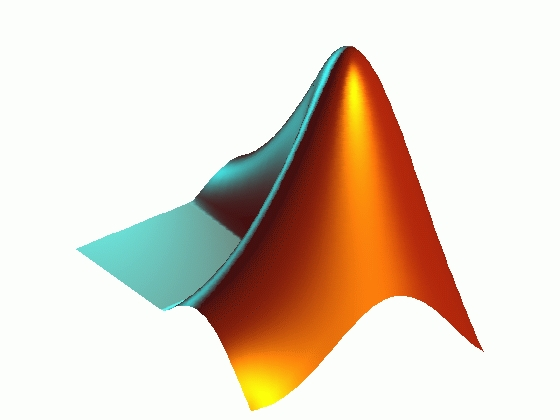
\includegraphics[scale=0.5]{figuraCapa2.jpg}
\vspace{3 cm}
}
\author{
\bf \sffamily \Large Abel Soares Siqueira (abel.s.siqueira@gmail.com) \\ 
\bf \Large \sffamily  Kally Chung (chung.kally@gmail.com) \\ 
}
\date{\bf \sffamily \large \today}

\numberwithin{equation}{section}

\renewcommand{\labelenumi}{\arabic{enumi}-}
\renewcommand{\labelenumii}{\arabic{enumi}.\arabic{enumii}-}
\renewcommand{\labelenumiii}{\arabic{enumi}.\arabic{enumii}.\arabic{enumiii}-}

\begin{document}

\pagestyle{empty}

\maketitle

\newpage

\tableofcontents

\newpage

\section*{Pref\'acio}

O Matlab (MATrix LABoratory) foi desenvolvido por Cleve Moler, do departamento de Ci\^encias da Computa\c{c}\~ao na Universidade do Novo M\'exico. Em 1983, o engenheiro Jack Little conheceu a linguagem Matlab e em se junta com Moler e Steve Bargert para, em 1984, fundar \textit{MathWorks} e comercializar Matlab.

Matlab foi inicialmente adotado por engenheiros e rapidamente se espalhou para outros campos de aplica\c{c}\~ao, tanto que, atualmente, \'e usado nas \'areas da educa\c{c}\~ao de \'Algebra Linear, An\'alise Num\'erica e tamb\'em na \'area de processamento de imagem.

O elemento b\'asico deste programa \'e uma matriz que n\~ao requer dimensionamento, facilitando a resolu\c{c}\~ao de muitos problemas num\'ericos uma vez que n\~ao precisamos ficar t\~ao preocupados em como passar as inst\^ancias e as sa\'{\i}das, nem como ajustar a dimens\~ao da matriz. Outro benef\'{\i}cio de se trabalhar com o Matlab \'e a facilidade de programar na linguagem dele e de construir gr\'aficos. Entretanto, j\'a que \'e f\'acil programar em Matlab, a desvantagem ocorre na falsa impress\~ao de que programar em outras linguagens \'e t\~ao f\'acil quanto no Matlab.

O Matlab foi desenvolvido inicialmente em C, por\'em hoje ele possui subrotinas em C, Fortran e Java, que s\~ao linguagens muito utilizadas, para que o usu\'ario n\~ao estranhasse a linguagem de programa\c{c}\~ao do Matlab.

Nesta apostila, queremos apresentar as fun\c{c}\~oes b\'asicas que funcionam em qualquer vers\~ao de Matlab, por\'em algumas mensagens de erro e de alerta podem ser diferentes por voc\^e estar trabalhando numa vers\~ao diferente ou numa plataforma diferente. 

Como j\'a fizemos uma breve introdu\c{c}\~ao sobre como o Matlab funciona, como ele chegou at\'e voc\^e, esperamos que voc\^e fa\c{c}a bom proveito da apostila, do curso e explore todos os recursos que o Matlab te oferece.

\begin{flushright}
Abel Soares Siqueira
\end{flushright}
\begin{flushright}
Kally Chung
\end{flushright}

\newpage

\section{\'Area de Trabalho do Matlab}
	Ao executar o Matlab, a Figura \ref{fig:area_trab_dest} fornece sua visualiza\c{c}\~ao padr\~ao. As partes destacadas correspondem, respectivamente, a \textit{(1)Janela de Comando}, \textit{(2)Hist\'orico de Comando}, \textit{(3)Espa\c{c}o de Trabalho} e \textit{(4)Diret\'orio Atual}, cujas aplica\c{c}\~oes s\~ao descritas na lista abaixo:
	
\begin{enumerate}
	\item \textit{Janela de Comando}: Principal local de intera\c{c}\~ao do usu\'ario com o Matlab porque \'e onde escrevemos os comandos, ap\'os o prompt {\tt >>}, para o Matlab executar. Quando o cursor \`a direita do prompt {\tt >>} ficar piscando, isso quer dizer que o Matlab est\'a esperando seu comando para execut\'a-lo.
	\item \textit{Hist\'orico de Comando}: Local de armazenamento dos comandos executados anteriormente na \textit{Janela de Comando}.
	\item \textit{Espa\c{c}o de Trabalho}: Apresenta\c{c}\~ao da lista das vari\'aveis criadas na sess\~ao atual de trabalho no MatLab.
	\item \textit{Diret\'orio Atual}: Respons\'avel pela manipula\c{c}\~ao dos diret\'orios e arquivos no Matlab.
\end{enumerate}
	
\begin{figure}[!h]
\centering
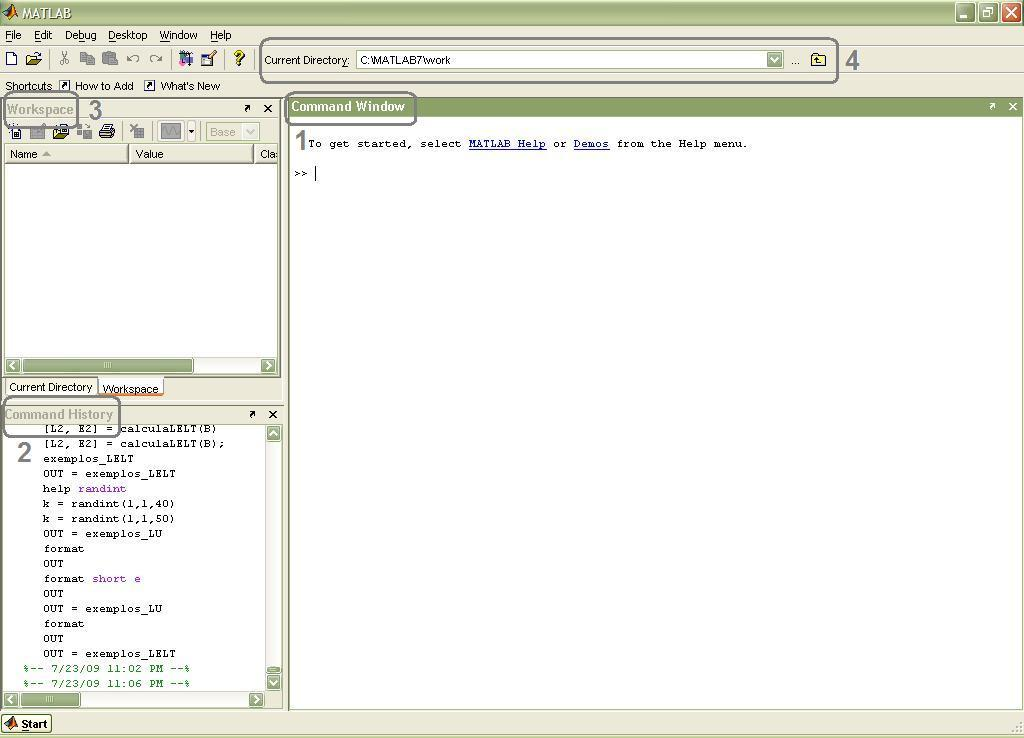
\includegraphics[scale=0.5]{figura2.jpg}
\caption{Visualiza\c{c}\~ao da \'area de trabalho do Matlab.}
\label{fig:area_trab_dest}
\end{figure}
	
	Como dito anteriormente, essa \'e uma \'area de trabalho padr\~ao uma vez que sua altera\c{c}\~ao \'e poss\'{\i}vel atrav\'es do menu superior {\tt Desktop}.

\newpage

\section{Inser\c{c}\~ao de Elementos B\'asicos}
	Neste cap\'{\i}tulo, trabalharemos somente na \textit{Janela de Comando} mostrando como inserir constantes, as quais incluem escalares, strings e n\'umeros complexos, e apresentando algumas fun\c{c}\~oes b\'asicas.

\subsection{Constantes}	
	
	Ao inserir uma constante ap\'os o prompt {\tt >>}, o Matlab ir\'a guard\'a-la na vari\'avel {\tt ans} e devolver\'a o resultado ap\'os a express\~ao {\tt ans =}. Note que logo ap\'os a execu\c{c}\~ao do comando, o \textit{Hist\'orico de Comando} j\'a \'e atualizado e a vari\'avel {\tt ans} aparece na lista de vari\'aveis do \textit{Espa\c{c}o de Trabalho}.
	
	Vejamos os exemplos abaixos sobre como introduzir escalar, string e n\'umeros complexos, respectivamente:
	
\begin{verbatim}
>> 14
ans =
    14
>> 5.27e-1
ans =
  5.2700e-001  
>> `Matlab'
ans =
Matlab
>> 8 - 2i
ans =
   8.0000 - 2.0000i
>> 8 - 2j
ans =
   8.0000 - 2.0000i   
>> ans
ans =
   8.0000 - 2.0000i 
\end{verbatim}	

	Ao saber qual valor que {\tt ans} armazena, \'e s\'o cham\'a-la. Vemos, no exemplo, que ela armazena a \'ultima constante inserida.

	Para introduzir uma string, basta escrever a palavra desejada entre aspas simples. J\'a para inserir um n\'umero complexo, a parte imagin\'aria pode ser acompanhada tanto de {\tt i} ou {\tt j}.

\subsection{Vari\'aveis}	

	Ao solicitar ao Matlab que guarde o resultado numa vari\'avel espec\'{\i}fica, j\'a n\~ao aparecer\'a {\tt ans} e, sim, o nome da vari\'avel especificada. A atualiza\c{c}\~ao tanto no \textit{Hist\'orico de Comandos} e no \textit{Espa\c{c}o de Trabalho} tamb\'em ocorrem.
	
\begin{verbatim}
>> total = 5+7*23
total =
   166
>> valor = 5.27e-1
valor =
  5.2700e-001
>> palavra = `Matlab'
palavra =
	Matlab
>> total_complexo = 4 + 3i + 0.7 + sin(0.5)*i
total_complexo =
   4.7000 + 3.4794i
\end{verbatim}		

\subsubsection{Regras para Trabalhar com as Vari\'aveis}
	Como estamos armazenando os dados em vari\'aveis, existem regras que devemos saber e obedecer.

\begin{enumerate}	
	\item As vari\'aveis distinguem letras mai\'usculas e min\'usculas. Por exemplo, as vari\'aveis {\tt Resultado, resultado, ReSuLtAdO} s\~ao diferentes para o Matlab.
	\item As vari\'aveis podem conter at\'e 31 caracteres que englobam letras, algarismos e sublinhados, portanto, caracteres de pontua\c{c}\~ao n\~ao s\~ao admitidos. Os nomes {\tt \$Resultado, Resul\$tado} n\~ao s\~ao aceitos como vari\'avel.
	\item O primeiro caractere de uma vari\'avel tem que ser letra. Nomes como {\tt 4resultado, \_resultado\_} n\~ao s\~ao admitidos como vari\'aveis.
	\item As vari\'aveis n\~ao podem pertencer ao conjunto das vari\'aveis reservadas pelo Matlab, o qual est\'a detalhado na Tabela \ref{tab:lista_reservadas}.
\end{enumerate}
	
\begin{table}[h]
\centering
\begin{tabular}{|c|c|c|c|c|c|} \hline	
{\tt for}    & {\tt end}   & {\tt if}        & {\tt while}      & {\tt function} & {\tt return} \\ \hline
{\tt elseif} & {\tt case}  & {\tt otherwise} & {\tt switch}     & {\tt continue} & {\tt else}   \\ \hline
{\tt try}    & {\tt catch} & {\tt global}    & {\tt persistent} & {\tt break}    &        \\ \hline
\end{tabular}
\caption{Vari\'aveis reservadas pelo Matlab.}
\label{tab:lista_reservadas}
\end{table}

\subsubsection{Vari\'aveis Pr\'e-Determinadas}
	A Tabela \ref{tab:lista_predef} apresenta algumas vari\'aveis pr\'e-determinadas. Embora sejam vari\'aveis pr\'e-determinadas, os nomes dessas vari\'aveis podem ser usados para armazenar outros valores.
	
\begin{table}[h]
\centering
\begin{tabular}{|c|l|} \hline	
\textbf{Vari\'avel}   & \textbf{Descri\c{c}\~ao} \\ \hline
{\tt pi}     & Valor de $\pi = 3.14159265358979...$ \\ \hline
{\tt inf}    & Valor de $\infty$, que representa o Infinito.   \\ \hline
{\tt NaN}    & Valor n\~ao num\'erico e significa \textit{Not a number}. \\ \hline
{\tt i} ou {\tt j} & Valor para $\sqrt{-1}$. \\ \hline
\end{tabular}
\caption{Vari\'aveis pr\'e-determinadas pelo Matlab.}
\label{tab:lista_predef}
\end{table}
	
\subsubsection{Oculta\c{c}\~ao das Solu\c{c}\~oes}	
	Voc\^e j\'a deve ter notado que ao digitar o comando, o Matlab executa e imprime o resultado. Entretanto, ao colocar ponto-e-v\'{\i}rgula no final do comando, o Matlab o executar\'a e n\~ao imprimir\'a o resultado. No exemplo abaixo, observe que a presen\c{c}a do ponto-e-v\'{\i}rgula nos 2 primeiros comandos oculta os resultados, que podem ser visualizados ao chamar a vari\'avel no prompt {\tt >>}.

\begin{verbatim}
>> total = 5+7*23;
>> valor = 5.27e-1;
>> total
total =
   166
>> valor
valor =
    0.5270
\end{verbatim}

\subsubsection{Uni\~ao de Comandos na \textit{Janela de Comando}}
	Podemos tamb\'em unir dois comandos por v\'{\i}rgula ou por ponto-e-v\'{\i}rgula. A v\'{\i}rgula, ao final do comando, n\~ao ocultar\'a o resultado, j\'a o ponto-e-v\'{\i}rgula, sim.
	
	Caso seu comando seja t\~ao longo que o apropriado seja quebr\'a-lo e continuar na linha seguinte, ent\~ao use retic\^encias (...) entre nomes de vari\'aveis e operadores matem\'aticos, e n\~ao no meio de vari\'aveis. Considere os exemplos abaixo:

\begin{verbatim}
>> valor1 = 5.4; valor2 = 9.3;
>> total = valor2/valor1
total =
    1.7222
>> total = valor2...
/valor1
total =
    1.7222
>> total = valor2/...
valor1
total =
    1.7222
>> total = valor...			%reticencias usadas no meio de uma variavel, por isso o erro
2/valor1
??? 2/valor1
    |
Error: Missing Matlab operator.
\end{verbatim}

\subsubsection{Comandos para Ministrar as Vari\'aveis}

	Existem comandos, os quais est\~ao listados na Tabela \ref{tab:lista_funcao_variaveis}, que nos auxiliam a administrar as vari\'aveis. Logo em seguida, alguns exemplos est\~ao expostos.
	
\begin{table}[h]
\centering
\begin{tabular}{|c|l|} \hline	
\textbf{Comando}   & \textbf{Descri\c{c}\~ao} \\ \hline
{\tt who}     & Lista das vari\'aveis existentes no Espa\c{c}o de Trabalho. \\ \hline
{\tt whos}    & Lista das vari\'aveis existentes, de suas dimens\~oes e seus tipos no Esp. de Trabalho. \\ \hline
{\tt clear}   & Remo\c{c}\~ao de pelo menos uma vari\'avel no Espa\c{c}o de Trabalho. \\ \hline
\end{tabular}
\caption{Comandos relacionados com administra\c{c}\~ao de vari\'aveis.}
\label{tab:lista_funcao_variaveis}
\end{table}

\begin{verbatim}
>> who
Your variables are:
A       B       C       M       c1      c2      c3      total   valor   valor2  
>> whos
  Name         Size                    Bytes  Class
  A            4x2                        64  double array
  B            2x3                        48  double array
  C            4x3                        96  double array
  M            4x2                        64  double array
  c1           1x1                        16  double array (complex)
  c2           1x1                        16  double array (complex)
  c3           1x1                        16  double array (complex)
  total        1x1                         8  double array
  valor        1x1                         8  double array
  valor2       1x1                         8  double array
Grand total is 40 elements using 344 bytes
>> clear c1
>> who
Your variables are:
A       B       C       M       c2      c3      total   valor   valor2  
>> clear M total
>> who
Your variables are:
A       B       C       c2      c3      valor   valor2 
>> clear		%apagando todas as variaveis
>> who			%jah nao aparece lista porque todas variaveis foram apagadas
\end{verbatim}

	Observe no exemplo que para apagar algumas vari\'aveis, basta list\'a-las ap\'os o comando clear. Por\'em para apagar todas as vari\'aveis, \'e s\'o usar o comando clear.
	
\subsection{Coment\'arios}
	Qualquer texto seguido do sinal de porcentagem torna-se um coment\'ario. Este n\~ao pode ser interrompido como se fosse um comando, logo, escreva o coment\'ario e caso este fique longo, quebre-o e continue a frase na linha seguinte, ap\'os digitar o sinal de porcentagem.
	
	No exemplo abaixo, o primeiro e o \'ultimo comando n\~ao geram erros, enquanto que os do meio geram porque o coment\'ario foi quebrado de forma errada, mesmo com o ``aux\'{\i}lio" das retic\^entias, que n\~ao funciona como ``continuador de comandos" porque o Matlab entende que elas fazem parte do coment\'ario j\'a que elas pertencem ao texto depois do sinal de porcentagem.
	
\begin{verbatim}
>> valor1 = 5.4; valor2 = 9.3;
>> total = valor2/valor1 %esse comando nao foi quebrado, nem o comentario
total =
    1.7222
>> total = valor2/valor1 %esse comando nao foi quebrado, mas
total =
    1.7222
>> o comentario sim
??? Undefined command/function 'o'.
>> total = valor2/valor1 %esse comando nao foi quebrado, mas...
total =
    1.7222
>>  o comentario sim
??? Undefined command/function 'o'.
>> total = valor2/valor1 %esse comando nao foi quebrado, mas...
total =
    1.7222
>> %o comentario sim
\end{verbatim}	

\newpage

\section{Visualiza\c{c}\~ao dos N\'umeros}
	Voc\^e deve ter notado que, at\'e agora, os resultados num\'ericos possuem 4 d\'{\i}gitos decimais. No entanto, essa formata\c{c}\~ao \'e alter\'avel. Veja outros formatos que o Matlab disponibiliza:
	
\begin{table}[h]
\centering
\begin{tabular}{|l|l|} \hline	
\textbf{Comando}     & \textbf{Descri\c{c}\~ao} \\ \hline
{\tt format short}   & 5 d\'{\i}gitos, com 4 d\'{\i}gitos decimais. \\ \hline
{\tt format long}    & 16 d\'{\i}gitos, com 15 d\'{\i}gitos decimais.   \\ \hline
{\tt format short e} & 5 d\'{\i}gitos, com 4 d\'{\i}gitos decimais, e expoente. \\ \hline
{\tt format long e}  & 16 d\'{\i}gitos, com 15 d\'{\i}gitos decimais, e expoente. \\ \hline
{\tt format short g} & Melhor formato dentre {\tt format short} e {\tt format short e}. \\ \hline
{\tt format long g}  & Melhor formato dentre {\tt format long} e {\tt format long e}. \\ \hline
{\tt format bank}    & 3 d\'{\i}gitos, com 2 d\'{\i}gitos decimais.  \\ \hline
\end{tabular}
\caption{Formatos de visualiza\c{c}\~ao dos n\'umeros.}
\label{tab:lista_formatos}
\end{table}

\begin{verbatim}
>> valor1 = 5.4; valor2 = 9.3;
>> total = valor2/valor1
total =
    1.7222  
>> format short
>> total
total =
    1.7222
>> format long
>> total
total =
   1.72222222222222
>> format short e
>> total
total =
  1.7222e+000
>> format long e
>> total
total =
    1.722222222222222e+000
>> format short g
>> total
total =
       1.7222
>> format long g
>> total
total =
          1.72222222222222
>> format bank
>> total
total =
          1.72
\end{verbatim}

\section{Fun\c{c}\~oes Matem\'aticas B\'asicas}

	Nas tabelas a seguir, apresentaremos as fun\c{c}\~oes comuns do Matlab, as quais podem ser aplicadas em MatLab's de outras vers\~oes e de outras plataformas.

\subsection{Opera\c{c}\~ao Elementar}

\begin{table}[h]
\centering
\begin{tabular}{|l|l|l|} \hline
\textbf{Comando} & \textbf{Descri\c{c}\~ao} & \textbf{Exemplo}    \\ \hline 
{\tt +}          & Adi\c{c}\~ao.         		& {\tt >> 43 + 4}  \\ \hline
{\tt -}          & Subtra\c{c}\~ao.     		& {\tt >> 43 - 4}  \\ \hline
{\tt *}          & Multiplica\c{c}\~ao. 		& {\tt >> 43 * 4}  \\ \hline
{\tt $\backslash$} ou {\tt /} & Divis\~ao.  & {\tt >> 43 / 4} ou {\tt >> 4 $\backslash$ 43} \\ \hline
{\tt $\widehat{}$}& Potencia\c{c}\~ao.   		& {\tt >> 43 $\widehat{}$ 4}  \\ \hline
\end{tabular}
\caption{Comandos do Matlab correspondente \`as opera\c{c}\~oes elementares.}
\label{tab:lista_oper_bas}
\end{table}

\subsection{Fun\c{c}\~ao Trigonom\'etrica}

\begin{table}[h]
\centering
\begin{tabular}{|l|l|l|} \hline
\textbf{Comando}     & \textbf{Descri\c{c}\~ao}     & \textbf{Exemplo}    \\ \hline 
{\tt sin}            & Seno.												& {\tt >> sin(pi/4)}  \\ \hline
{\tt cos}            & Cosseno.                     & {\tt >> cos(pi/4)}  \\ \hline
{\tt tan}            & Tangente.                    & {\tt >> tan(pi/4)}  \\ \hline
{\tt csc}         	 & Cosecante.                   & {\tt >> csc(pi/4)}  \\ \hline
{\tt sec}		         & Secante. 								    & {\tt >> sec(pi/4)}  \\ \hline
%comandos arco
{\tt asin}   				 & Arco Seno.  						 		 	& {\tt >> asin(7.0711e-1)}  \\ \hline
{\tt acos}   				 & Arco Cosseno.  					 		& {\tt >> acos(7.0711e-1)}  \\ \hline
{\tt atan}   				 & Arco Tangente.  				 		  & {\tt >> atan(7.0711e-1)}  \\ \hline
{\tt acsc}           & Arco Cosecante.          		& {\tt >> acsc(1.4142)}  \\ \hline
{\tt asec}           & Arco Secante. 					      & {\tt >> asec(1.4142)}  \\ \hline
%comandos hiperbolico
{\tt sinh}					 & Seno Hiperb\'olico.			 		& {\tt >> sinh(log(10))}  \\ \hline
{\tt cosh}					 & Cosseno Hiperb\'olico.	 		  & {\tt >> cosh(log(10))}  \\ \hline
{\tt tanh}					 & Tangente Hiperb\'olico.  		& {\tt >> tanh(log(10))}  \\ \hline
{\tt csch}		       & Cosecante Hiperb\'olica.     & {\tt >> csch(log(10))}  \\ \hline
{\tt sech}           & Secante Hiperb\'olica.       & {\tt >> sech(log(10))}  \\ \hline
%comandos arco hiperbolico
{\tt asinh}					 & Arco Seno Hiperb\'olico.     & {\tt >> asinh(4.9500)}  \\ \hline
{\tt acosh}					 & Arco Cosseno Hiperb\'olico.  & {\tt >> acosh(5.05)}  \\ \hline
{\tt atanh}					 & Arco Tangente Hiperb\'olico. & {\tt >> atanh(9.8020e-1)}  \\ \hline
{\tt acsch}		       & Arco Cosecante Hiperb\'olica.& {\tt >> acsch(2.0202e-1)}  \\ \hline
{\tt asech}          & Arco Secante Hiperb\'olica.  & {\tt >> asech(1.9802e-1)}  \\ \hline
\end{tabular}
\caption{Comandos do Matlab correspondente \`as fun\c{c}\~oes trigonom\'etricas.}
\label{tab:lista_trig}
\end{table}

\newpage
\subsection{Fun\c{c}\~ao Exponencial e Logar\'{\i}tmica}

\begin{table}[h]
\centering
\begin{tabular}{|l|l|l|} \hline
\textbf{Comando} & \textbf{Descri\c{c}\~ao}    & \textbf{Exemplo}    \\ \hline 
{\tt exp}       	& Exponencial.							 & {\tt >> exp(1)}  \\ \hline
{\tt log}         & Logaritmo Natural $(=ln)$. & {\tt >> log(2.7183)}  \\ \hline
{\tt log10}       & Logaritmo na Base 10.      & {\tt >> log10(1000)}  \\ \hline
{\tt log2}        & Logaritmo na Base 2.       & {\tt >> log2(1024)}  \\ \hline
{\tt sqrt}	      & Raiz Quadrada.						 & {\tt >> sqrt(36)}  \\ \hline
\end{tabular}
\caption{Comandos do Matlab correspondente \`as fun\c{c}\~oes exponenciais e logar\'{\i}tmicas.}
\label{tab:lista_exp_log}
\end{table}

\subsection{Fun\c{c}\~ao Complexa}

\begin{table}[h]
\centering
\begin{tabular}{|l|l|l|} \hline
\textbf{Comando}  & \textbf{Descri\c{c}\~ao}            & \textbf{Exemplo}    \\ \hline 
{\tt abs}         & Valor Absoluto ou M\'odulo.	 				& {\tt >> abs(-4)} ou {\tt >> abs(-4+6*i)}  \\ \hline
{\tt angle}       & \^Angulo de fase em radianos.				& {\tt >> angle(-4+6*i)}  \\ \hline
{\tt conj}        & Conjugado Complexo.          				& {\tt >> conj(-4+6*i)}  \\ \hline
{\tt imag}        & Parte Imagin\'aria.          				& {\tt >> imag(-4+6*i)}  \\ \hline
{\tt real}	      & Parte Real.   							 				& {\tt >> real(-4+6*i)}  \\ \hline
{\tt isreal}	    & Verdadeiro(1) para valores reais, falso(0) caso contr\'ario.	& {\tt >> isreal(-4+6*i)}  \\ \hline
\end{tabular}
\caption{Comandos do Matlab correspondente \`as fun\c{c}\~oes complexas.}
\label{tab:lista_complexa}
\end{table}

\subsection{Fun\c{c}\~ao de Arredondamento e de Resto}

\begin{table}[h]
\centering
\begin{tabular}{|l|l|l|} \hline
\textbf{Comando}  & \textbf{Descri\c{c}\~ao}                      & \textbf{Exemplo}    \\ \hline 
{\tt fix}         & Arredondamento na dire\c{c}\~ao de zero.      & {\tt >> fix(-7.6010)}  \\ \hline
{\tt floor}       & Fun\c{c}\~ao Ch\~ao.                          & {\tt >> floor(7.6010)}  \\ \hline
{\tt ceil}        & Fun\c{c}\~ao Teto.                            & {\tt >> ceil(7.6010)}  \\ \hline
{\tt round}       & Arredondamento para o inteiro mais pr\'oximo. & {\tt >> round(7.6010)}  \\ \hline
{\tt mod}	        & Resto da divis\~ao com sinal.                 & {\tt >> mod(7.6010,-3)}  \\ \hline
{\tt rem}	        & Resto da divis\~ao.                           & {\tt >> rem(7.6010,3)}  \\ \hline
{\tt sign}	      & Fun\c{c}\~ao Sinal.                           & {\tt >> sign(-7.6010)}  \\ \hline
\end{tabular}
\caption{Comandos do Matlab correspondente \`as fun\c{c}\~oes de arredondamentos e de restos.}
\label{tab:lista_arred_resto}
\end{table}

\newpage

\subsection{Fun\c{c}\~ao de Convers\~ao}

\begin{table}[h]
\centering
\begin{tabular}{|l|l|l|} \hline
\textbf{Comando}  & \textbf{Descri\c{c}\~ao}            	& \textbf{Exemplo}    \\ \hline 
{\tt deg2rad}     & Convers\~ao de graus para radianos.	  & {\tt >> deg2rad(45)}  \\ \hline
{\tt rad2deg}     & Convers\~ao de radianos para graus.   & {\tt >> rad2deg(pi/4)}  \\ \hline
\end{tabular}
\caption{Comandos do Matlab correspondente \`as fun\c{c}\~oes de convers\~ao.}
\label{tab:lista_conversao}
\end{table}

\subsection{Usando {\tt Help}}

	Quando surgir alguma d\'uvida sobre comandos, fun\c{c}\~oes, quais argumentos s\~ao necess\'arios para uma dada fun\c{c}\~ao, use o comando {\tt Help}, que est\'a exemplificado abaixo:

\begin{verbatim}	
>> help mod
 MOD    Modulus after division.
    MOD(x,y) is x - n.*y where n = floor(x./y) if y ~= 0.  If y is not an
    integer and the quotient x./y is within roundoff error of an integer,
    then n is that integer.  By convention, MOD(x,0) is x.  The input
    x and y must be real arrays of the same size, or real scalars.
 
    The statement "x and y are congruent mod m" means mod(x,m) == mod(y,m).
 
    MOD(x,y) has the same sign as y while REM(x,y) has the same sign as x.
    MOD(x,y) and REM(x,y) are equal if x and y have the same sign, but
    differ by y if x and y have different signs.
 
    See also rem.

    Overloaded functions or methods (ones with the same name in other directories)
       help sym/mod.m

    Reference page in Help browser
       doc mod

>> help sqrt
 SQRT   Square root.
    SQRT(X) is the square root of the elements of X. Complex 
    results are produced if X is not positive.
 
    See also sqrtm.

    Overloaded functions or methods (ones with the same name in other directories)
       help sym/sqrt.m

    Reference page in Help browser
       doc sqrt
\end{verbatim}

\section{Vetores}
	At\'e agora, lidamos com constantes, informa\c{c}\~oes individuais. Mas, neste cap\'{\i}tulo, concatenamos esses dados individuais em vetor e veremos como aplicar as opera\c{c}\~oes para eles sem aplicar a opera\c{c}\~ao de um em um.
	
	O Matlab interpreta um vetor como uma matriz de uma linha e v\'arias colunas e n\~ao uma estrutura com v\'arias linhas e uma coluna, como em \'Algebra Linear. Da mesmo forma que quando t\'{\i}nhamos uma constante, o Matlab tratava-a como uma matriz de uma linha e uma coluna.

\subsection{Cria\c{c}\~ao de Vetores}

	Vamos mostrar, nas pr\'oximas se\c{c}\~oes, cinco maneiras de criar vetores. Existe um modo direto de cria\c{c}\~ao, um que determinamos o primeiro e o \'ultimo elemento, outro que determinamos o primeiro elemento e o n\'umero de componentes no vetor e o \'ultimo m\'etodo que cria vetores de vetores.

\subsubsection{Modo Direto de Cria\c{c}\~ao de Vetor}
	Uma vez que voc\^e j\'a conhece os elementos os quais comp\~oem o seu vetor, coloque, entre colchetes, os elementos separados por espa\c{c}os ou v\'{\i}rgulas. Por exemplo:
	
\begin{verbatim}
>> u = [0.95013  0.76210  0.61543  0.40571  0.57891]
u =
    0.9501    0.7621    0.6154    0.4057    0.5789
>> u2 = [0.95013,  0.76210,  0.61543,  0.40571,  0.57891]
u2 =
    0.9501    0.7621    0.6154    0.4057    0.5789
\end{verbatim}

\subsubsection{Progress\~ao Aritm\'etica com Raz\~ao 1}
	Para criar um vetor cujos componentes s\~ao consecutivos, basta usar a express\~ao
\begin{center}
{\tt <In\'{\i}cio> : <Final>}
\end{center}

O Matlab entender\'a que voc\^e deseja criar um vetor cujo primeiro elemento \'e {\tt <In\'{\i}cio>} e os pr\'oximos elementos ser\~ao incrementados em $1$ e p\'ara no elemento mais pr\'oximo de {\tt <Final>}.

\begin{verbatim}
>> u1 = 1:4
u1 =
     1     2     3     4
>> v = -1:11
v =
    -1     0     1     2     3     4     5     6     7     8     9    10    11     
>> z = 2.5:8.4
z =
    2.5000    3.5000    4.5000    5.5000    6.5000    7.5000     
\end{verbatim}	
	
\subsubsection{Progress\~ao Aritm\'etica com Raz\~ao $\neq$ 1}

	Usando a express\~ao
\begin{center}	
{\tt <In\'{\i}cio> : <Incremento> : <Final>}
\end{center}
o Matlab entender\'a que voc\^e deseja construir um vetor a partir de {\tt <In\'{\i}cio>} e os pr\'oximos ser\~ao incrementados de {\tt <Incremento>} at\'e que alcance ao elemento mais pr\'oximo de {\tt <Final>}, como nos exemplos abaixo:

\begin{verbatim}
>> u = -1:3:11
u =
    -1     2     5     8    11
    
>> v = 14:-2:2
v =
    14    12    10     8     6     4     2

>> z = 4.5:2.3:19.4
z =
    4.5000    6.8000    9.1000   11.4000   13.7000   16.0000   18.3000    
\end{verbatim}

\subsubsection{Vetor com N\'umero de Elementos Definidos}

	A express\~ao
\begin{center}	
{\tt linspace ( <In\'{\i}cio> : <Final> : <NumElementos> )}
\end{center}
devolver\'a um vetor que come\c{c}a em {\tt <In\'{\i}cio>}, termina em {\tt <Final>} e possui {\tt <NumElementos>} componentes.

\begin{verbatim}
>> u = linspace(-1,3.5,5)
u =
           -1        0.125         1.25        2.375          3.5
>> v = linspace(15,-pi,8)
v =
           15       11.372       7.7434        4.115      0.48673      -3.1416
\end{verbatim}

	J\'a a express\~ao 
\begin{center}	
{\tt logspace ( <In\'{\i}cio> : <Final> : <NumElementos> )}
\end{center}
difere da anterior porque cria espa\c{c}amentos logar\'{\i}tmicos entre seus elementos aos inv\'es de espa\c{c}amentos lineares. 

	O Matlab, ao efetuar o comando {\tt logspace}, entende que o usu\'ario deseja criar um vetor, de {\tt <NumElementos>} que come\c{c}a em $10^{Inicio}$ e termina em $10^{Final}$.

\begin{verbatim}
>> v = logspace(0,2,5)
v =
            1       3.1623           10       31.623          100
\end{verbatim}

\subsubsection{Jun\c{c}\~ao de Vetores}
	Um vetor tamb\'em pode ser, vamos dizer, recriado ao juntar dois ou mais vetores.

\begin{verbatim}
>> u = [0.4447 0.61543 0.79194];
>> u2 = [0.92181 0.73821 0.17627 0.40571];
>> v = [u u2]
v =
       0.4447      0.61543      0.79194      0.92181      0.73821      0.17627      0.40571
\end{verbatim}

\subsection{Orienta\c{c}\~ao de Vetores}
	Sabe-se que o vetor definido por \'Algebra Linear e pelo Matlab s\~ao diferentes, por\'em, para escrever um vetor em p\'e, basta usar ponto-e-v\'{\i}rgula entre cada um dos elementos ou transpor um vetor deitado.
	
\begin{verbatim}	
>> u = [0.4447; 0.61543; 0.79194]
u =
       0.4447
      0.61543
      0.79194
\end{verbatim}	

	Outras maneiras de transpor um vetor linha para um vetor coluna:
\begin{verbatim}	
>> a = 3:6
a =
     3     4     5     6
>> a_t = a'
a_t =
     3
     4
     5
     6
>> a_t2 = a.'
a_t2 =
     3
     4
     5
     6
>> b = 1 + a*i
b =
   1.0000 + 3.0000i   1.0000 + 4.0000i   1.0000 + 5.0000i   1.0000 + 6.0000i
>> b_t = b'
b_t =
   1.0000 - 3.0000i
   1.0000 - 4.0000i
   1.0000 - 5.0000i
   1.0000 - 6.0000i
>> b_t2 = b.'
b_t2 =
   1.0000 + 3.0000i
   1.0000 + 4.0000i
   1.0000 + 5.0000i
   1.0000 + 6.0000i
\end{verbatim}

	Se o seu vetor \'e formado por elementos reais, podemos realizar a transposi\c{c}\~ao usando o operador de transposi\c{c}\~ao(') ou o operador de transposi\c{c}\~ao pontuada(.'). Por\'em se o seu vetor \'e composto por n\'umeros imagin\'arios, o operador de transposi\c{c}\~ao transp\~oe e conjuga enquanto que o operador de transposi\c{c}\~ao pontuada somente transp\~oe.
	
	Outra fato a considerar, no exemplo, \'e que para definir o vetor $b$, adiciono o n\'umero $1$ a um vetor multiplicado com sua parte imagin\'aria. Em outras linguagens de programa\c{c}\~ao, n\~ao podemos somar dois tipos diferentes, mas neste caso, Matlab \'e ``inteligente" para perceber que esse 1 \'e como um vetor de `uns'.

\subsection{Endere\c{c}amento Vetorial}

	Para obter um certo elemento num dado vetor, digite o nome do vetor e entre par\^entesis o \'{\i}ndice desejado.
No entanto, se \'e necess\'ario ter acesso a pelo menos um elemento, ent\~ao podemos usar uma estrutura vetorial v\'alida no argumento dentro do par\^entesis.	Por exemplo:
	
\begin{verbatim}
>> v = [0.4447		0.61543		0.79194		0.92181		0.73821		0.17627		0.40571		0.93547];
>> v(5)
ans =
    0.7382
>> v(6:end)
ans =
    0.1763    0.4057    0.9355
>> v([6 7 8])
ans =
    0.1763    0.4057    0.9355
>> v([6 6 7 8])
ans =
    0.1763    0.1763    0.4057    0.9355
\end{verbatim}

\newpage

\section{Matrizes}

	Ao introduzir vetores, foi dito que o Matlab l\^e um vetor como uma matriz de uma linha e v\'arias colunas, assim, os comandos para vetores s\'o tinham que se preocupar com a dimens\~ao da coluna. Agora, veremos que esses comando ser\~ao ajustados para matrizes porque temos duas dimens\~oes para tratar, linha e coluna.

	A partir daqui em diante, vamos definir que se alguma fun\c{c}\~ao \'e v\'alida para matrizes, ela tamb\'em \'e v\'alida para vetores.	
	
\subsection{Inser\c{c}\~ao de Matrizes}
	Numa matriz, o que separa uma linha da outra \'e o ponto-e-v\'{\i}rgula ou ``enter". Mostraremos quatro modos de inserir um vetor, mas existem outras maneiras para isso.
	
\begin{verbatim}	
>> A = [1 2 3; 4 5 6; 7 8 9]
A =
     1     2     3
     4     5     6
     7     8     9
>> B = [1 2 3
4 5 6
7 8 9 ]
B =
     1     2     3
     4     5     6
     7     8     9
>> C = [1, 2, 3
4, 5, 6,
7, 8, 9 ]
C =
     1     2     3
     4     5     6
     7     8     9  
>> D = [1:3;4:6;7:9]
D =
     1     2     3
     4     5     6
     7     8     9     
\end{verbatim}

	Observe que cada linha de uma matriz \'e tratada como um vetor, ent\~ao desde que usemos um comando v\'alido para escrever essa linha e separando ou com ponto-e-v\'{\i}rgula ou enter, temos uma matriz.
	
	Note que as express\~oes abordadas para criar um vetor, como
\begin{center}
{\tt <In\'{\i}cio> : <Final>} \\
{\tt <In\'{\i}cio> : <Incremento> : <Final>} \\
{\tt linspace ( <In\'{\i}cio> : <Final> : <NumElementos> )} \\
{\tt logspace ( <In\'{\i}cio> : <Final> : <NumElementos> )} \\
\end{center}
n\~ao podem ser aplicadas para toda uma matriz, mas podem ser aplicadas de linha para linha de uma matriz.

	No entanto, a estrat\'egia de criar vetores juntando vetores tamb\'em \'e v\'alida para matrizes, desde as dimens\~oes sejam compat\'{\i}veis. Vejamos:
\begin{verbatim}	
>> E = rand(3)
E =
    0.4447    0.9218    0.4057
    0.6154    0.7382    0.9355
    0.7919    0.1763    0.9169
>> F = [A E]
F =
    1.0000    2.0000    3.0000    0.4447    0.9218    0.4057
    4.0000    5.0000    6.0000    0.6154    0.7382    0.9355
    7.0000    8.0000    9.0000    0.7919    0.1763    0.9169    
\end{verbatim}

	Em {\tt >> E =  rand(3)} do exemplo acima, criamos uma matriz de 3 linhas por 3 colunas cujas componentes s\~ao geradas aleatoriamente.
	
\subsection{Orienta\c{c}\~ao de Matrizes}
	O operador de transposi\c{c}\~ao (') e o de transposi\c{c}\~ao pontuada(.') trabalham de forma id\^entica ou com vetor ou com matrizes, como mostrado no exemplo:
\begin{verbatim}	
>> A = [1 2 3; 4 5 6; 7 8 9]
A =
     1     2     3
     4     5     6
     7     8     9
>> B = rand(3)+i*rand(3)
B =
   0.6602 + 0.3704i   0.3412 + 0.4449i   0.3093 + 0.7948i
   0.3420 + 0.7027i   0.5341 + 0.6946i   0.8385 + 0.9568i
   0.2897 + 0.5466i   0.7271 + 0.6213i   0.5681 + 0.5226i
>> A_t = A'
A_t =
     1     4     7
     2     5     8
     3     6     9
>> A_t2 = A.'
A_t2 =
     1     4     7
     2     5     8
     3     6     9
>> B_t = B'
B_t =
   0.6602 - 0.3704i   0.3420 - 0.7027i   0.2897 - 0.5466i
   0.3412 - 0.4449i   0.5341 - 0.6946i   0.7271 - 0.6213i
   0.3093 - 0.7948i   0.8385 - 0.9568i   0.5681 - 0.5226i
>> B_t2 = B.'
B_t2 =
   0.6602 + 0.3704i   0.3420 + 0.7027i   0.2897 + 0.5466i
   0.3412 + 0.4449i   0.5341 + 0.6946i   0.7271 + 0.6213i
   0.3093 + 0.7948i   0.8385 + 0.9568i   0.5681 + 0.5226i
\end{verbatim}
	
\subsection{Opera\c{c}\~oes com Escalares}

	J\'a mostramos um exemplo anteriormente na qual realizamos uma soma de um escalar com um vetor. Por\'em, esse comando ``inteligente'' n\~ao se restringe a soma, mas tamb\'em para subtra\c{c}\~ao, multiplica\c{c}\~ao e divis\~ao. O caso da multiplica\c{c}\~ao e da divis\~ao por escalar s\~ao os mais conhecidos porque s\~ao semelhantes \`a opera\c{c}\~ao alg\'ebrica.
	
	A Tabela \ref{tab:lista_oper_mat_esc} detalha as opera\c{c}\~oes que podemos realizar com matrizes e escalares.

\begin{table}[h]
\centering
\begin{tabular}{|l|l|} \hline
\textbf{Comando} 									& \textbf{Descri\c{c}\~ao}   \\ \hline 
{\tt A + c}      									& Soma do escalar {\tt c} com todos os elementos da matriz {\tt A}.  \\ \hline
{\tt A - c}      									& Subtra\c{c}\~ao do escalar {\tt c} com todos os elementos da matriz {\tt A}. \\ \hline
{\tt A*c} ou {\tt c*A}  					& Multiplica\c{c}\~ao do escalar {\tt c} com todos os elementos da matriz {\tt A}. \\ \hline
{\tt A/c} ou {\tt c$\backslash$A} & Divis\~ao do escalar {\tt c} com todos os elementos da matriz {\tt A}.  \\ \hline
\end{tabular}
\caption{Comandos do Matlab correspondente \`as opera\c{c}\~oes matriciais com escalares.}
\label{tab:lista_oper_mat_esc}
\end{table}

\subsection{Opera\c{c}\~oes entre Matrizes}

	A Tabela \ref{tab:lista_oper_mat_bas} apresenta as opera\c{c}\~oes elementares dispon\'{\i}veis para matrizes, j\'a supondo que elas t\^em dimens\~oes compat\'{\i}veis.

\begin{table}[h]
\centering
\begin{tabular}{|l|l|} \hline
\textbf{Comando} 			& \textbf{Descri\c{c}\~ao}    			\\ \hline 
{\tt +}      					& Soma de matrizes.                 \\ \hline
{\tt -}      					&	Subtra\c{c}\~ao de matrizes.      \\ \hline
{\tt *}        				& Multiplica\c{c}\~ao de matrizes.  \\ \hline
{\tt $\widehat{}$}    & Potencia\c{c}\~ao de matrizes.    \\ \hline
\end{tabular}
\caption{Comandos do Matlab correspondente \`as opera\c{c}\~oes elementares com matrizes.}
\label{tab:lista_oper_mat_bas}
\end{table}

\begin{verbatim}	
>> A = [1 2 3; 4 5 6; 7 8 9];
>> B = rand(3)
B =
    0.4447    0.9218    0.4057
    0.6154    0.7382    0.9355
    0.7919    0.1763    0.9169
>> A + B
ans =
    1.4447    2.9218    3.4057
    4.6154    5.7382    6.9355
    7.7919    8.1763    9.9169
>> A - B
ans =
    0.5553    1.0782    2.5943
    3.3846    4.2618    5.0645
    6.2081    7.8237    8.0831
>> A^2
ans =
    30    36    42
    66    81    96
   102   126   150
>> A*A
ans =
    30    36    42
    66    81    96
   102   126   150
>> A*B
ans =
    4.0514    2.9270    5.0274
    9.6076    8.4359   11.8016
   15.1638   13.9447   18.5758
\end{verbatim}
	
O Matlab tamb\'em oferece opera\c{c}\~oes elemento a elemento, que s\~ao realizados pelos operadores pontuados. Um operador pontuado j\'a visto \'e o de transposi\c{c}\~ao pontuada(.').

\begin{table}[h]
\centering
\begin{tabular}{|l|l|} \hline
\textbf{Comando} 								& \textbf{Descri\c{c}\~ao}  							   \\ \hline 
{\tt .*}         								& Multiplica\c{c}\~ao elemento a elemento.   \\ \hline
{\tt .$\backslash$} ou {\tt ./} & Divis\~ao de elemento a elemento.   			 \\ \hline
{\tt .$\widehat{}$}   					& Potencia\c{c}\~ao de elemento a elemento.  \\ \hline
{\tt .'}                        & Transposi\c{c}\~ao de elemento a elemento. \\ \hline
\end{tabular}
\caption{Comandos do Matlab correspondente \`as opera\c{c}\~oes matriciais de elemento a elemento.}
\label{tab:lista_oper_mat_elem_elem}
\end{table}
	
\begin{verbatim}
>> A = [1 2 3; 4 5 6; 7 8 9];
>> M = [1 1 1;2 2 2;3 3 3];
>> A.*M
ans =
     1     2     3
     8    10    12
    21    24    27
>> A./M
ans =
    1.0000    2.0000    3.0000
    2.0000    2.5000    3.0000
    2.3333    2.6667    3.0000
>> A.^M
ans =
     1     2     3
    16    25    36
   343   512   729
\end{verbatim}

\subsection{Fun\c{c}\~oes Especiais para Criar Matrizes Padr\~ao}

	Matriz padr\~ao inclui matriz identidade, matrizes de n\'umeros aleat\'orios, matrizes nulas e matrizes de `uns'.

\begin{table}[h]
\centering
\begin{tabular}{|l|l|} \hline
\textbf{Fun\c{c}\~ao} & \textbf{Descri\c{c}\~ao}  							  \\ \hline 
{\tt eye(n)}     			& Matriz Identidade de dimens\~ao {\tt n}. \\ \hline
{\tt eye(l,c)}   			& Matriz com {\tt l} linhas e {\tt c} colunas tal que $A(i,i) = 1$ e $A(i,j) = 0$, $i \neq j$. \\ \hline 
{\tt ones(n)}    			& Matriz de dimens\~ao {\tt n} com todos os elementos iguais a um.  \\ \hline
{\tt ones(l,c)}  			& Matriz com {\tt l} linhas e {\tt c} colunas com todos os elementos iguas a um.  \\ \hline
{\tt zeros(n)}   			& Matriz de dimens\~ao {\tt n} com todos os elementos iguas a zero.  \\ \hline
{\tt zeros(l,c)} 			& Matriz com {\tt l} linhas e {\tt c} colunas com todos os elementos iguas a zero.  \\ \hline
{\tt rand(n)}    			& Matriz de dimens\~ao {\tt n} de n\'umeros aleat\'orios com elementos entre 0 e 1. \\ \hline
{\tt rand(l,c)}  			& Matriz com {\tt l} linhas e {\tt c} de n\'umeros aleat\'orios com elementos entre 0 e 1.  \\ \hline
\end{tabular}
\caption{Fun\c{c}\~oes para criar matrizes padr\~ao.}
\label{tab:lista_mat_padrao}
\end{table}

\begin{verbatim}	
>> eye(4)
ans =
     1     0     0     0
     0     1     0     0
     0     0     1     0
     0     0     0     1
>> zeros(1,5)
ans =
     0     0     0     0     0
>> ones(2,3)
ans =
     1     1     1
     1     1     1
\end{verbatim}

\subsection{Endere\c{c}amento Matricial}

	O endere\c{c}amento matricial funciona da mesma maneira que no caso de vetores, com a difere\c{c}a de ajuste de argumentos, ou seja, para fazer refer\^encia a um elemento da matriz, precisamos indical qual a linha e qual a coluna. Entretanto, a manipula\c{c}\~ao desses argumentos \'e o mesmo que para vetor. Vejamos os exemplos:
	
\begin{verbatim}	
>> A = [1 2 3; 4 5 6; 7 8 9];		%definindo a matriz
>> A(3,2)
ans =
     8
>> A(1:2,1:3) 	%buscando a primeira e segunda linha e da primeira ateh a ultima coluna
ans =
     1     2     3
     4     5     6
>> A(:,2)		%buscando todas as linhas e a segunda coluna
ans =
     2
     5
     8
>> A(3:-1:1,:)		%buscando da terceira ateh primeira linha, todas as colunas
ans =
     7     8     9
     4     5     6
     1     2     3
>> A(3:-1:2,1:2)		%buscando da terceira ateh segunda linha e da primeira ateh segunda coluna
ans =
     7     8
     4     5
\end{verbatim}

	O operador dois-pontos representa ou todas as linhas ou todas as colunas, dependendo de onde est\'a posicionado o operador. Nos exemplos, veja que se o operador aparece no primeiro argumento, ent\~ao queremos selecionar todas as linhas, contudo, se o operador aparece no segunda argumento, queremos selecionar todas as colunas.
	
	A Tabela \ref{tab:lista_oper_mat_end} abaixo mostra alguns comandos para endere\c{c}amento matricial.
	
\begin{table}[h]
\centering
\begin{tabular}{|l|l|} \hline
\textbf{Comando}  & \textbf{Descri\c{c}\~ao}    \\ \hline 
{\tt A(r,c)}      & Devolve a submatriz {\tt A} cujas linhas e colunas s\~ao definidas por {\tt r} e {\tt c}. \\ \hline
{\tt A(r,:)}      & Devolve a submatriz {\tt A} cujas linhas s\~ao definidas por {\tt r} e com todas as colunas.  \\ \hline
{\tt A(:,c)}      & Devolve a submatriz {\tt A} cujas colunas s\~ao definidas por {\tt c} e com todas as linhas.  \\ \hline
{\tt A(:)}        & Devolve todos os elementos de {\tt A} em um vetor coluna, coluna a coluna.  \\ \hline
\end{tabular}
\caption{Comandos do Matlab correspondentes \`a endere\c{c}amento matricial.}
\label{tab:lista_oper_mat_end}
\end{table}
	
	Tendo $A(:)$, estamos trabalhando com um vetor, sendo assim, podemos usar os recursos de endere\c{c}amento vetorial para $A(:)$.

\subsection{Mais Recursos Dispon\'{\i}veis para Matrizes}

\begin{table}[h]
\centering
\begin{tabular}{|l|l|} \hline
\textbf{Fun{c}\~ao} & \textbf{Descri\c{c}\~ao}    \\ \hline 
{\tt sort(A)}     	& Ordena\c{c}\~ao das colunas da matriz {\tt A}.  \\ \hline
{\tt sort(A,1)}   	& Ordena\c{c}\~ao ao longo da primeira dimens\~ao (linha).  \\ \hline
{\tt sort(A,2)}   	& Ordena\c{c}\~ao ao longo da segunda dimens\~ao (linha).  \\ \hline
{\tt find(x)}     	& Devolve os \'{\i}ndices que satisfazem condi\c{c}\~ao {\tt x}.  \\ \hline
{\tt max(A)}      	& Devolve o m\'axima de cada coluna de {\tt A}.  \\ \hline
{\tt min(A)}      	& Devolve o m\'{\i}nimo de cada coluna de {\tt A}.  \\ \hline
\end{tabular}
\caption{Mais fun\c{c}\~oes para matrizes.}
\label{tab:lista_oper_mat_outros}
\end{table}

	Todos os comandos acima podem ter um ou dois argumentos de sa\'{\i}da. Para o caso de ordena\c{c}\~ao, m\'aximo ou m\'{\i}nimo, o primeiro argumento \'e solu\c{c}\~ao do comando, j\'a o segundo argumento \'e referente ao \'{\i}ndice da ordena\c{c}\~ao, m\'aximo ou m\'{\i}nimo.
	No caso do {\tt find}, uma sa\'{\i}da retorna a posi\c{c}\~ao do vetor, por\'em duas sa\'{\i}das exibem a linha e a coluna da matriz. Veja os exemplos:

\begin{verbatim}
>> B = rand(3)
B =
    0.4447    0.9218    0.4057
    0.6154    0.7382    0.9355
    0.7919    0.1763    0.9169 
>> [C,id] = sort(B)
C =
    0.4447    0.1763    0.4057
    0.6154    0.7382    0.9169
    0.7919    0.9218    0.9355
id =
     1     3     1
     2     2     3
     3     1     2    
>> v = find(B>0.5)
v =
     2
     3
     4
     5
     8
     9
>> [idv,jdv] = find(B>0.5)
idv =
     2
     3
     1
     2
     2
     3
jdv =
     1
     1
     2
     2
     3
     3
>> [u,idu] = max(B)
u =
    0.7919    0.9218    0.9355
idu =
     3     1     2
>> [u2,idu2] = min(B)
u2 =
    0.4447    0.1763    0.4057
idu2 =
     1     3     1     
\end{verbatim}

\newpage

\subsection{Dimens\~oes de Matrizes}
	
\begin{table}[h]
\centering
\begin{tabular}{|l|l|} \hline
\textbf{Fun\c{c}\~ao} & \textbf{Descri\c{c}\~ao}\\ \hline 
{\tt size(A)} 		    & Retorna as dimens\~oes da matriz {\tt A}.  \\ \hline
{\tt size(A,1)}   		& Retorna n\'umero de linhas de {\tt A}.  \\ \hline
{\tt size(A,2)} 		  & Retorna n\'umero de colunas de {\tt A}.  \\ \hline
{\tt length(A)}   		& Retorna o comprimento de {\tt A}.  \\ \hline
{\tt numel(A)}    		& Retorna o n\'umero total de elementos de {\tt A}.  \\ \hline
\end{tabular}
\caption{Fun\c{c}\~oes relacionadas a dimensionamento de matrizes.}
\label{tab:lista_dimensao}
\end{table}

\subsection{Fun\c{c}\~oes de \'Algebra Matricial}

\begin{table}[h]
\centering
\begin{tabular}{|l|l|} \hline
\textbf{Fun\c{c}\~ao}   & \textbf{Descri\c{c}\~ao}\\ \hline 
{\tt A$\widehat{}$ n}   & Potenciac\~ao de matrizes.  \\ \hline
{\tt det(A)}   				  & Determinante de {\tt A}.  \\ \hline
{\tt inv(A)}   					& Inversa de {\tt A}.  \\ \hline
{\tt cond(A)}   				& N\'umero de condi\c{c}\~ao de {\tt A}.  \\ \hline
{\tt rank(A)} 					& Posto de {\tt A}.  \\ \hline
{\tt diag(A)} 					& Vetor que guarda os elementos da diagonal principal de {\tt A}.  \\ \hline
{\tt diag(diag(A))} 		& Matriz que guarda os elementos da diagonal principal de {\tt A}.  \\ \hline
\end{tabular}
\caption{Fun\c{c}\~oes relacionadas a \'Algebra Matricial.}
\label{tab:lista_algebra}
\end{table}		
	
\newpage	
	
\section{Programando no Matlab}
	Vimos que \'e poss\'{\i}vel trabalhar com mais de um comando num mesmo prompt {\tt >>} desde que separemos os comandos com v\'{\i}rgula ou ponto-e-v\'{\i}rgula. Por\'em, caso desejamos executar uma sequ\^encia de comandos, a Janela de Comandos j\'a n\~ao seria conveniente e assim, podemos recorrer ao Editor do Matlab, que armazenam esses sequ\^encias de comandos nos arquivos ``.m''.
	
	Existem duas maneiras de acessar o Editor do Matlab, as quais est\~ao ilustradas nas figuras abaixo. A primeira \'e clicando em \textbf{``New M-File''}, que est\'a representado por uma p\'agina em branco no toolbar do Matlab. A segunda maneira \'e atrav\'es da barra de ferramentas, em File $\rightarrow$ New $\rightarrow$ M-file.

\begin{figure}[!h]
\centering
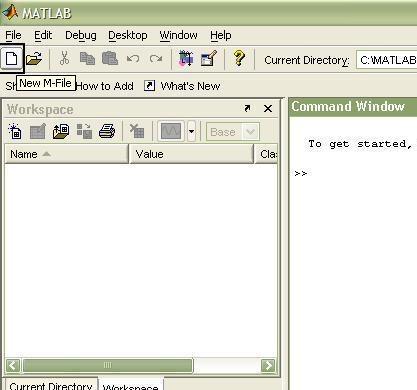
\includegraphics[scale=0.5]{figura3.jpg} \qquad
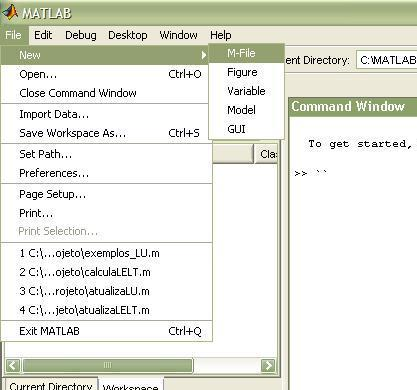
\includegraphics[scale=0.5]{figura4.jpg}
\caption{Os dois modos de acesso para os Arquivos M.}
\label{fig:acesso_editor}
\end{figure}

\begin{enumerate}
	\item Mesmo o Matlab tendo o seu editor, n\~ao \'e necess\'ario que o programa seja escrito nesse editor, por\'em \'e preciso que o arquivo seja salvo com extens\~ao ``.m''.
	\item A primeira linha de comando do seu arquivo M \'e 
\begin{center}	
{\tt function[<vari\'aveis\_de\_sa\'{\i}da>] = <nome\_da\_fun\c{c}\~ao>(<vari\'aveis\_de\_entrada>)}
\end{center}
	Se o seu programa retornar somente uma vari\'avel de sa\'{\i}da, ent\~ao os colchetes s\~ao opcionais; se o seu programa n\~ao tem vari\'aveis de entrada, os par\^entesis s\~ao opcionais; se o seu programa n\~ao tem vari\'aveis de entrada e de sa\'{\i}da, o cabe\c{c}alho acima tamb\'em n\~ao \'e necess\'ario, no entanto, se quiser permanecer com o cabe\c{c}alho, use a express\~ao abaixo:
\begin{center}	
{\tt function <nome\_da\_fun\c{c}\~ao>}
\end{center}	

Para chamar seu arquivo M, v\'a na \textit{Janela de Comando}, chame seu arquivo M atrav\'es da express\~ao
\begin{center}	
{\tt >> [<vari\'aveis\_de\_sa\'{\i}da\_desejadas>]=<nome\_da\_fun\c{c}\~ao>(<vari\'aveis\_de\_entrada>)}
\end{center}
ou
\begin{center}	
{\tt >> <nome\_da\_fun\c{c}\~ao>}
\end{center}
onde a primeira express\~ao se refere aos casos em que existem ou vari\'aveis de entrada ou de sa\'{\i}da e a segunda aos que n\~ao existe nem vari\'aveis de sa\'{\i}da nem de entrada.

Se o seu algoritmo exibe tr\^es vari\'aveis de sa\'{\i}da, ent\~ao no Matlab, n\~ao \'e necess\'ario que se chame todas essas tr\^es vari\'aveis, somente as que o usu\'ario necessitar.

	\item Salve seu arquivo M com o mesmo nome da fun\c{c}\~ao. Ent\~ao, se o nome da fun\c{c}\~ao \'e {\tt teste}, salve seu arquivo como {\tt teste.m}
	\item Os nomes de fun\c{c}\~ao devem come\c{c}ar com letra. O uso de letras, n\'umeros e sublinhados devem ser colocados ap\'os a primeira letra.
	\item Atualize o diret\'orio onde est\~ao os seus arquivos M.
	\item As primeiras linhas de coment\'ario antes ou abaixo	do cabe\c{c}alho do {\tt function} ser\~ao interpretadas pelo Matlab como help do seu arquivo M.
\end{enumerate}
	
\subsection{Exemplos}

\subsubsection{Cria\c{c}\~ao de Vetores}

	Vamos criar o vetor abaixo:

\begin{table}[h]
\centering
\begin{tabular}{|c|c|c|c|c|c|c|c|c|c|c|} \hline
$0$ & $0.1\pi$ & $0.2\pi$ & $0.3\pi$ & $0.4\pi$ & $0.5\pi$ & $0.6\pi$ & $0.7\pi$ & $0.8\pi$ & $0.9\pi$ & $\pi$ \\ \hline
\end{tabular}
\caption{Vetor a ser criado para exemplificar como trabalhar com arquivos M.}
\label{tab:exemplo_arquivoM}
\end{table}			
	
\begin{verbatim}	
%criando_vetor.m
%primeira maneira de criar o vetor proposto
%uma funcao que nao tem variaveis de entrada, mas tem variaveis de saida
function v = criando_vetor

v = 0:0.1:1;
v = pi*v;
\end{verbatim}
\line(1,0){200}
\begin{verbatim}	
%criando_vetor2.m
%segunda maneira de criar o vetor proposto
%uma funcao que nao tem variaveis de entrada nem de saida

v = [0 0.1*pi 0.2*pi 0.3*pi 0.4*pi 0.5*pi 0.6*pi 0.7*pi 0.8*pi 0.9*pi pi]
\end{verbatim}
\line(1,0){200}
\begin{verbatim}	
%criando_vetor.m
%terceira maneira de criar o vetor proposto
%uma funcao que nao tem variaveis de entrada, mas tem variaveis de saida
function v = criando_vetor3

v = linspace(0,pi,11);
\end{verbatim}	

No Matlab,
\begin{verbatim}
>> v = criando_vetor
v =
		0		0.3142		0.6283		0.9425		1.2566		1.5708		1.8850		2.1991		2.5133		2.8274		3.1416
>> criando_vetor2
v =
		0		0.3142		0.6283		0.9425		1.2566		1.5708		1.8850		2.1991		2.5133		2.8274		3.1416
>> help criando_vetor
 criando_vetor.m
 primeira maneira de criar o vetor proposto
 uma funcao que nao tem variaveis de entrada, mas tem variaveis de saida
\end{verbatim} 

\subsubsection{Realizando a Divis\~ao}

	Dado um n\'umero a e b, vamos realizar a divis\~ao de a por b e retornar o quociente e o resto.
	
\begin{verbatim}	
%divisao.m
%realiza divisao de a por b
%variaveis de entrada: a e b
%variaveis de saida: quoc e resto (referente a quociente e resto)
function [quoc,resto] = divisao(a,b)

quoc = a/b;
quoc = floor(quoc);
resto = a - b*quoc;
\end{verbatim}
\line(1,0){200}
\begin{verbatim}
%divisao2.m
%realiza divisao de a por b
%variaveis de entrada: a e b
%nao tem variaveis de saida

function divisao2(a,b)

quoc = a/b;
quoc = floor(quoc)
resto = a - b*quoc
\end{verbatim}

No Matlab, fazendo a chamada de {\tt divisao.m} e {\tt divisao2.m}, respectivamente.
\begin{verbatim}
>> [quoc,resto] = divisao(15,4)
quoc =
     3
resto =
     3
>> divisao2(15,2)
quoc =
     7
resto =
     1     
\end{verbatim}

\newpage

\section{Operadores Relacionais e L\'ogicos}	
	Os operadores relacionais e l\'ogicos s\~ao respons\'aveis por fornecer respostas do tipo Falso/Verdeiro a perguntas. Se a resposta for verdadeira, o operador retorna 1, por\'em se a resposta for falsa, ent\~ao operador	devolve 0. 
	
\subsection{Operadores Relacionais}	
	
\begin{table}[h]
\centering
\begin{tabular}{|l|l|} \hline
\textbf{Comando} & \textbf{Descri\c{c}\~ao}    \\ \hline 
{\tt $<$}    		 & Menor que. \\ \hline
{\tt $\leq$}     & Menor ou igual a. \\ \hline
{\tt $>$}     	 & Maior que. \\ \hline
{\tt $\geq$}     & Maior ou igual a. \\ \hline
{\tt $==$}       & Igualdade, usado em compara\c{c}\~ao. \\ \hline
{\tt $\sim=$}    & Diferente de, usado em compara\c{c}\~ao.  \\ \hline
\end{tabular}
\caption{Comandos de Operadores Relacionais.}
\label{tab:lista_oper_relacional}
\end{table}		

	Vejamos os exemplos para aplicar o operador relacional. Al\'em de obter respostas para perguntas por meio de operador relacional, podemos combinar express\~oes relacionais com express\~oes matem\'aticas, como mostra o \'ultimo exemplo.
	
\begin{verbatim}
>> A = rand(1,4)
A =
    0.8913    0.7621    0.4565    0.0185
>> B = rand(1,4)
B =
    0.8214    0.4447    0.6154    0.7919
>> vf = A > B
vf =
     1     1     0     0
>> vf = B - (A > 0.6)
vf =
   -0.1786   -0.5553    0.6154    0.7919
\end{verbatim}

\subsection{Operadores L\'ogicos}

\begin{table}[h]
\centering
\begin{tabular}{|l|l|} \hline
\textbf{Comando} & \textbf{Descri\c{c}\~ao}    \\ \hline 
{\tt \&}		     & E, usado em compara\c{c}\~ao de senten\c{c}as. \\ \hline
{\tt $\vert$}    & OU, usado em compara\c{c}\~ao de senten\c{c}as. \\ \hline
{\tt $\sim$}     & N\~AO, usado em compara\c{c}\~ao de senten\c{c}as. \\ \hline
\end{tabular}
\caption{Comandos de Operadores L\'ogicos.}
\label{tab:lista_oper_logico}
\end{table}		

\begin{verbatim}
>> vfn = ~(A > B)
vfn =
     0     0     1     1
>> vfc = (A > 0.5) & (B > 0.5)
vfc =
     1     0     0     0
\end{verbatim}

\subsection{Fun\c{c}\~oes Relacionais e L\'ogicos}

\begin{table}[h]
\centering
\begin{tabular}{|l|l|} \hline
\textbf{Comando} & \textbf{Descri\c{c}\~ao}    \\ \hline 
{\tt xor(x,y)}   & OU Exclusivo.  \\ \hline
{\tt any(x)}     & Retorna verdadeiro se algum elemento satisfaz a condi\c{c}\~ao {\tt x}. \\ \hline
{\tt all(x)}     & Retorna falso se todos elementos satisfazem a condi\c{c}\~ao {\tt x}. \\ \hline
\end{tabular}
\caption{Fun\c{c}\~oes relacionais e l\'ogicos.}
\label{tab:lista_func_relac_logico}
\end{table}		

	O OU Exclusivo funciona da seguinte maneira: retorna verdadeiro(1) se uma das duas condi\c{c}\~oes forem verdadeiras e falso(0) se ambas condi\c{c}\~oes s\~ao falsas ou verdadeiras.
	
\begin{verbatim}
>> all(A>0.5)
ans =
     0
>> any(A>0.5)
ans =
     1
\end{verbatim}

\newpage

\section{Controle de Fluxo}

	Controle de fluxo \'e a habilidade de ajustar a maneira como um programa realiza suas tarefas. Por meio de instru��es especiais, chamadas comandos, essas tarefas podem ser executadas seletivamente ou repetidamente.

\subsection{Estrutura For}

	O loop for sequencia uma s\'erie de comandos por um n\'umero de vezes fixo e predefinido. A estrutura geral \'e:
	
\begin{verbatim}
for i = vetor
    comandos...
end	
\end{verbatim}
Para cada coluna do vetor i, os comandos interiores do for s\~ao realizados. Veja os exemplos:

\begin{verbatim}
function [x,y] = programa1

for i = 1:10
    x(i) = sin(i*pi/10);
end
for j = 10:-1:1
    y(j) = sin(j*pi/10);
end
\end{verbatim}
\line(1,0){200}
\begin{verbatim}
%i representa o contador do loop for no programa 2
function [i,x] = programa2

i = 0;
for n = (1:10)'
    i = i+1;
    x(n) = sin(n*pi/10);
end
\end{verbatim}
\line(1,0){200}
\begin{verbatim}
%i representa o contador do loop for no programa 3
%y criada somando a coluna da matriz que vai no contador
function [i,y] = programa3

i = 0;
for x = eye(4,5)
    i = i + 1;
    y(i) = sum(x);
end
\end{verbatim}
No Matlab:
\begin{verbatim}
>> [x,y] = programa1
x =
		0.30902		0.58779		0.80902		0.95106		      1		0.95106		0.80902		0.58779		0.30902		1.2246e-016
y =
		0.30902		0.58779		0.80902		0.95106		      1		0.95106		0.80902		0.58779		0.30902		1.2246e-016
>> [i,x] = programa2			
i =
     1			
x =		
		0.30902		0.58779		0.80902		0.95106		      1		0.95106		0.80902		0.58779		0.30902		1.2246e-016
>> [i,y] = programa3			
i =
     5
y =
     1     1     1     1     0		
\end{verbatim}

Note, nos exemplos mostrados, que no {\tt vetor} da estrutura {\tt for}, podemos colocar vetor linha, vetor coluna ou at\'e matriz, por\'em o que \'e usado como contador do loop for \'e o n\'umero de colunas de {\tt vetor}.

\'E recomend\'avel que os vetores sejam pr\'e-alocados antes que um loop {\tt for} ou {\tt while} comece porque se reduzem as opera\c{c}\~oes de aloca\c{c}\~ao de mem\'oria exigidas. Assim, durante o loop, somente a altera\c{c}\~ao de valores no vetores \'e realizada. Vamos fazer a altera\c{c}\~ao no {\tt programa1.m} para exemplificar.

\begin{verbatim}
% programa1.m modificado
function [x,y] = programa1_mod

%exemplos de como jah podemos pre-alocar os vetores usados no programa
x = zeros(1,10);
y = ones(1,10);

for i = 1:10
    x(i) = sin(i*pi/10);
end
for j = 10:-1:1
    y(j) = sin(j*pi/10);
end
\end{verbatim}

\subsection{Estrutura while}

\begin{verbatim}
while condicao
    comandos...
end
\end{verbatim}

	Pela forma geral da estrutura while, mostrada acima, podemos concluir que a continuidade do loop while depende da veracidade de todos os elementos de {\tt condicao} e n\~ao de um n\'umero pr\'e-fixado. Seguem os exemplos:

\begin{verbatim}
function i = programa4(num)

i = 0;
while ( num > 1)
    i = i + 1;
    num = num/2;
end
\end{verbatim}

	No Matlab, fazendo a chamada:

\begin{verbatim}
>> i = programa4(45)
i =
     6
>> i = programa4(16)
i =
     4
\end{verbatim}	

\subsection{Estrutura If-Else}

	Essas estruturas j\'a n\~ao s\~ao loops, ou seja, os comandos ser\~ao executados somente uma vez condicionalmente. A estrutura mais simples \'e
	
\begin{verbatim}
if condicao
     comandos...
end
\end{verbatim}
Os {\tt comandos...} ser\~ao executados se a {\tt condicao} for satisfeita.

	Se existem mais condi\c{c}\~oes para avaliar, ent\~ao a estrutura passa a ser:
\begin{verbatim}
if condicao1
     comandos1...
else
     comandos2...
end
\end{verbatim}
Neste caso, se {\tt condicao1} \'e verdadeira, ent\~ao os {\tt comandos1...} ser\~ao realizados; se {\tt condicao1} \'e falsa, ent\~ao os {\tt comandos2...} ser\~ao realizados. Apesar de n\~ao ter nenhuma {\tt condicao} a ser avaliada no else, o Matlab j\'a entende que a express\~ao ao ser avaliada no {\tt else} \'a a nega\c{c}\~ao de {\tt condicao1}.

	Mas mesmo assim, se existirem mais que duas condi\c{c}\~oes para serem avaliadas, ent\~ao a estrutura aumenta se tornando:

\begin{verbatim}
if condicao1
     comandos1...
elseif condicao2
     comandos2...
elseif condicao3
     ...
...
     ...	     
else
     comandos_finais...
end
\end{verbatim}
Nessa \'ultima estrutura, o {\tt else} n\~ao \'e necess\'ario, ou seja, podemos usar somente o {\tt if} e {\tt elseif}'s. O funcionamento ocorre similar \`as estruturas anteriores, isto \'e, a execu\c{c}\~ao dos comandos dependem da veracidade da {\tt condicao} a que eles est\~ao submetidos. Vejamos os exemplos:
\begin{verbatim}
%funcao que diz se o numero num eh par ou impar
%se vf = 1, entao num eh par
%se vf = 0, entao num eh impar
function vf = eh_par(num)

if ( rem(num,2) == 0 )
    vf = 1;
else
    vf = 0;
end
\end{verbatim}
\line(1,0){200}	
\begin{verbatim}
%programando a funcao sinal
%sinal = 1 se num � positivo
%sinal = -1 se num � negativo
%sinal = 0 se num = 0
function sinal = f_sinal(num)

sinal = 0;
if num > 0
    sinal = 1;
elseif num < 0
    sinal = -1;
end
\end{verbatim}

No Matlab:
\begin{verbatim}
>> vf = eh_par(5)
vf =
     0
>> sinal = f_sinal(-2)
sinal =
    -1
>> sinal = f_sinal(43)
sinal =
     1
\end{verbatim}

\subsection{Estrutura Switch-Case}

	A estrutura, mostrada acima, tem o mesmo funcionamento que o {\tt if-else}, mas a diferen\c{c}a \'e que no {\tt if-else} verifica se a condi\c{c}\~ao \'e verdadeira ou n\~ao e no switch-case verifica a igualdade da {\tt teste\_expressao}. 

	No {\tt switch-case}, a expressao pode ser um escalar ou uma string. Se {\tt expressao} \'e igual a {\tt teste\_expressao1}, ent\~ao executam-se os {\tt comandos1...} e j\'a vai direto no {\tt end}, no entanto, se {\tt expressao} \'e diferente de {\tt teste\_expressao1}, faz o teste de igualdade com {\tt teste\_expressao2} e assim por diante.

\begin{verbatim}
switch expressao
     case teste_expressao1
          comandos1...
     case teste_expressao2
          comandos2...
     case teste_expressao3
          ...
     ...
          ...               
     otherwise
          comandos_finais...
end
\end{verbatim}

	Exemplos:
\begin{verbatim}
function y = conversao(x, unidades)

switch unidades
    case {'polegadas','pol'}
        y = x*2.54;
    case {'pes','p'}
        y = x*2.54/12;        
    case {'metros','m'}    
        y = x/100;
    case {'milimetros','mm'}        
        y = x*10;
    case {'centimetros','cm'}
        y = x;
    otherwise
        disp(['Unidade desconhecida: ' unidades])
        y = nan;
end
\end{verbatim}

No Matlab:
\begin{verbatim}
>> y = conversao(5.2, 'akjd')
Unidade desconhecida: akjd
y =
   NaN
>> y = conversao(5.2, 'm')
y =
        0.052
\end{verbatim}

\subsection{Comandos para Interromper Loops}

	O comando {\tt break} interrompe o loop em que ele est\'a inserido e continua a compilar o arquivo M ap\'os a primeira linha fora do loop no qual ele aparece. Esse comando pode ser usado nas estruturas {\tt if-else}, {\tt for} e {\tt while}.

	O comando {\tt continue}, que \'e usado no {\tt for} e {\tt while}, faz com que o Matlab v\'a direto para a instru\c{c}\~ao final do loop, ignorando todos os comando entre o {\tt continue} e o {\tt end} e assim, segue com a pr\'oxima itera\c{c}\~ao. Podemos tamb\'em usar continue no {\tt if-else}, por\'em esse comando n\~ao tem efeito porque o {\tt if-else} s\'o tem uma itera\c{c}\~ao.
	
	J\'a o comando {\tt return} p\'ara a execu\c{c}\~ao do arquivo M. Quando o comando {\tt return} \'e encontrado no arquivo M, mesmo que esteja dentro de um loop, o Matlab j\'a avan\c{c}a para a \'ultima linha.
	
	Seguem os exemplos abaixo:
	
\begin{verbatim}		
%Essa funcao recebe o numero num
%Enquanto num+1 eh maior que um, num vai sendo dividido por 2.
%Quando num+1 eh menor que um, multiplica num por 2 e termina o loop.
function [num,i] = programa5(num)

for i = 1:1000
    num = num/2;
    if (1+num <= 1)
        num = 2*num;
        break
    end
end
\end{verbatim}
\line(1,0){200}	
\begin{verbatim}
%funcao que recebe um numero num
%se num for par, dividir por 2
%se nao, multiplicar por 3 e somar com 1
%o loop continua ateh que num seja 1
function i = programa6(num)

for i = 1:1000
    if (num == 1)
        return
    end
    if (eh_par(num) == 1)
        num = num/2;
    else
        num = num*3+1;
    end
end
\end{verbatim}
	
	Lembre-se que � fun\c{c}\~ao {\tt eh\_par} foi usado como um exemplo anterior para mostrar como trabalhar com a estrutura {\tt if-else}.
	
	Veja, no	exemplo, que a primeira fun\c{c}\~ao gera uma sequ\^encia de n\'umeros tal que o \'ultima elemento \'e zero, enquanto que a segunda fun\c{c}\~ao gera uma sequ\^encia de n\'umeros cujo \'ultimo elemento \'e um. 
	Perceba que quando {\tt num} atinge o valor do \'ultimo elemento, a leitura do arquivo M \'e finalizada e o Matlab retorna as vari\'aveis de sa\'{\i}da que foram obtidas at\'e que ele se encontrasse com o {\tt break} e {\tt return}.
	
\subsection{Recurs\~ao}

	Recurs\~ao \'e um m\'etodo de programa\c{c}\~ao no qual uma fun\c{c}\~ao pode chamar a si mesma, como por exemplo: N\'umeros de Fibonacci, N\'umero Fatorial.
	
	Lembra da fun\c{c}\~ao {\tt programa6(num)}, que recebe um n\'umero que \'e dividido por 2 se ele for par ou multiplicado por 3 e somado com 1 se ele for \'{\i}mpar. Apresentamos essa fun\c{c}\~ao por meio da estrutura for, agora vamos program\'a-lo usando recurs\~ao.
	
\begin{verbatim}
%funcao que usa recursao
%recebe um numero num
%se num for par, dividir por 2
%se nao, multiplicar por 3 e somar com 1
%o loop continua ateh que num seja 1
function i = programa6_recursao(num,i)

if (num == 1)
    return
end

if (eh_par(num) == 1)
    i = programa6_recursao(num/2, i)+1;
else
    i = programa6_recursao((3*num+1)/2, i)+2;
end
\end{verbatim}
	
\subsection{Fun\c{c}\~oes como Argumento}	
	Passar fun\c{c}\~oes como argumento n\~ao \'e t\~ao simples porque estamos passando uma string, por\'em precisamos transformar essa string numa express\~ao de comando v\'alida.

\subsubsection{Comando Eval}
	Este comando recebe uma string e recorre a um interpretador do Matlab que avalia qualquer string que se adapte \`a sintaxe do Matlab. Em se tratando de fun\c{c}\~oes como argumento, o comando {\tt eval} atende bem \`as nossas necessidades.
	
\begin{verbatim}	
>> x = 1; y = 3;
>> a = eval('x^2 + y^2')
a =
    10
>> b = eval('100*(y-x^2)^2 + (1-x)^2')
b =
   400
>> c = eval('eh_par(15)')
c =
     0   
\end{verbatim}
	
	Ao recorrer ao {\tt eval} para interpretar uma string como comando, se exige bastante do computador. Ent\~ao, podemos usar o comando {\tt feval} para diminuir a frequ\^encia do uso de {\tt eval}.
	
\subsubsection{Comando feval}	
	Este comando tem sua opera\c{c}\~ao limitada em rela\c{c}\~ao ao {\tt eval}, por\'em \'e mais eficiente porque o Matlab j\'a sup\~oe que o usu\'ario est\'a passando uma fun\c{c}\~ao do Matlab como argumento. Para se usar {\tt feval},
	
\begin{center}	
{\tt feval(`minha\_funcao',x)}
\end{center}
	
	Por exemplo, na \textit{Janela de Comando}:
\begin{verbatim}	
>> feval(`exp',2)
ans =
    7.3891
>> exp(2)
ans =
    7.3891    
>> feval(`x+1',4)
??? Error using ==> feval
Invalid function name `x+1'.
\end{verbatim}

Por\'em, outra alternativa para passar fun\c{c}\~ao como argumento \'e function\_handle, que \'e uma ferramenta ainda mais eficiente.

\subsubsection{Function\_Handle}
	O function\_handle \'e mais eficiente que os comandos anteriores porque \'e como se o Matlab criasse um arquivo M com a fun\c{c}\~ao passada como argumento e calculasse o valor da fun\c{c}\~ao para um ponto ou vetor dado. Portanto, o function\_handle \'e mais direto no que precisamos e n\~ao estamos limitados pelas fun\c{c}\~oes do Matlab, mas pode ser qualquer express\~ao matem\'atica.

Na \textit{Janela de Comando}:
\begin{verbatim}
>> f = @(x) exp(x)
f = 
    @(x) exp(x)
>> f(2)
ans =
    7.3891
>> g = @(x,y) (x^2+y^2)
g = 
    @(x,y) (x^2+y^2)
>> g(1,3)
ans =
    10
>> feval(g,1,3)
ans =
    10
>> feval(@(x,y) (x^2+y^2),1,3)
ans =
    10        
\end{verbatim}

Exemplo em um arquivo M:

\begin{verbatim}
function x = programa7(funcao,x)

for i = 1:length(x)
    x(i) = feval(funcao,x(i));
end    
\end{verbatim}

E da\'{\i}, chamando na \textit{Janela de Comando}, temos:	
\begin{verbatim}
>> funcao = @(x) (x^2-1)
funcao = 
    @(x) (x^2-1)
>> x = programa7(funcao,[1 2 3])
x =
     0     3     8  
>> x = programa7(`x^2-1',[1 2 3])
??? Invalid function name `x^2-1'.

Error in ==> programa7 at 4
    x(i) = feval(funcao,x(i));         
\end{verbatim}
	
	O feval s\'o funciona quando o argumento \'e uma fun\c{c}\~ao, ou seja, algum arquivo M. Nesse caso, {\tt `$x^2$-1'} n\~ao est\'a numa fun\c{c}\~ao, mas {\tt funcao = @(x) ($x^2$-1)} \'e um fun\c{c}\~ao\_handle, por isso que o feval executa o comando.
	
\newpage	
	
\section{Gr\'aficos Bidimensionais}	
	Uma das vantagens de se trabalhar com Matlab \'e a versatilidade para gerar e trabalhar com gr\'aficos, al\'em da extensa op\c{c}\~oes e fun\c{c}\~oes relacionadas com gr\'aficos.

\subsection{Conhecendo a fun\c{c}\~ao {\tt plot}} 
	O comando {\tt plot} \'e o comando mais comum para a elabora\c{c}\~ao de gr\'aficos bidimensionais. Os dois primeiros argumentos que v\~ao no comando {\tt plot} s\~ao, respectivamente os pontos da abscissa e os da ordenada. Da\'{\i}, o Matlab plota os pontos e conecta-os com retas. Veja o exemplo:
	
\begin{verbatim}	
>> x = rand(2,6)
x =
    0.4057    0.9169    0.8936    0.3529    0.0099    0.2028
    0.9355    0.4103    0.0579    0.8132    0.1389    0.1987
>> plot(x(1,:),x(2,:))
\end{verbatim}
	
	O gr\'afico obtido \'e:
\begin{figure}[!h]
\centering
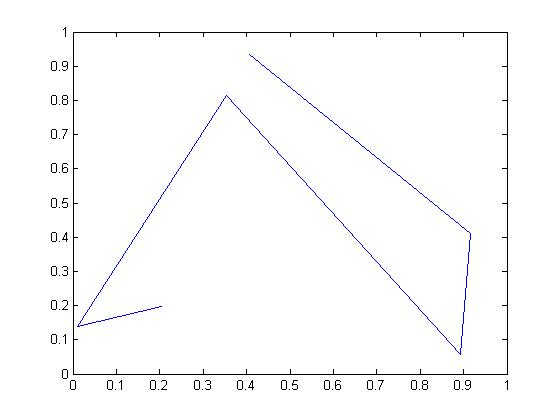
\includegraphics[scale=0.5]{grafico1.jpg}
\caption{Gr\'afico do primeiro exemplo de {\tt plot}.}
\label{fig:graf_bd1}
\end{figure}
	
Se quisermos plotar mais de uma fun\c{c}\~ao num mesmo gr\'afico, \'e s\'o continuar colocando os vetores no argumento de plot.
\begin{verbatim}
>> x = linspace(0,2*pi,30);
>> y = -1.1+0.4*x;
>> z = cos(x);
>> plot(x,y,x,z), title(`Grafico com duas funcoes')
\end{verbatim}	

O gr\'afico adquirido \'e:
\begin{figure}[!h]
\centering
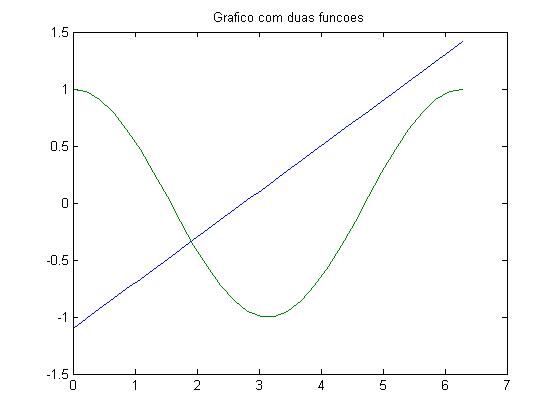
\includegraphics[scale=0.4]{grafico2.jpg}
\caption{Gr\'afico com duas fun\c{c}\~oes.}
\label{fig:graf_bd2}
\end{figure}

\subsection{Estilos de Linhas, Marcadores e Cores}

	No Matlab, tamb\'em \'e poss\'{\i}vel alterar o estilo da linha do gr\'afico, at\'e mesmo para facilitar a visualiza\c{c}\~ao, caso voc\^e tenha que plotar mais de uma reta. 
	
	As informa\c{c}\~oes espec\'{\i}ficas sobre qual o tipo de linha, marcador e cores s\~ao mostradas no terceiro argumento. Confira a Tabela \ref{tab:lista_estilos} abaixo para saber quais os estilos que voc\^e pode usar. Vamos usar o \'ultimo	gr\'afico mostrado para exemplificar como colocar estilos:
	
\begin{verbatim}	
>> plot(x,y,`r-',x,z,`b-.')
>> title(`Trabalhando estilos de linhas')
>> xlabel(`eixo das abscissas'), ylabel(`eixo das ordenadas')
\end{verbatim}	
\begin{figure}[!h]
\centering
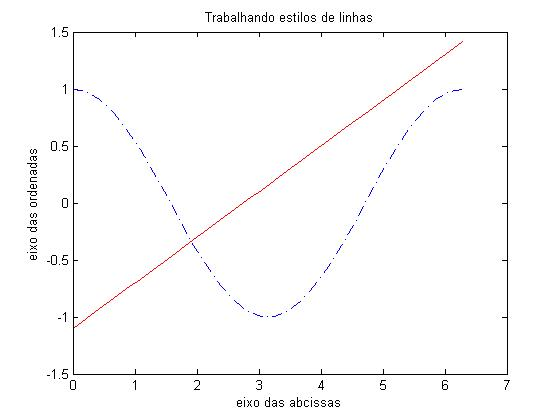
\includegraphics[scale=0.4]{grafico3.jpg}
\caption{Gr\'afico com estilo de linhas.}
\label{fig:graf_bd_3}
\end{figure}	

\newpage

\begin{table}[h]
\centering
\begin{tabular}{|l|l|l|l|l|l|} \hline	
\textbf{S\'{\i}mbolo} & \textbf{Cor} & \textbf{S\'{\i}mbolo} & \textbf{Marcador} & \textbf{S\'{\i}mbolo} & \textbf{Tipo de Linha} \\ \hline
{\tt b} & Azul & . & Ponto & - & Linha Cont\'{\i}nua \\ \hline
{\tt g} & Verde & o & C\'{\i}rculo & : & Linha pontilhada \\ \hline
{\tt r} & Vermelho & x & Cruz & -. & Tra\c{c}os e Pontos \\ \hline
{\tt c} & Ciano & + & Sinal de Positivo & - - & Linha tracejada \\ \hline
{\tt m} & Magenta & * & Estrela ou Asterisco & & \\ \hline
{\tt y} & Amarelo & s & Quadrado & & \\ \hline
{\tt k} & Preto & d & Losango & & \\ \hline
{\tt w} & Branco & v & Tri\^angulo para baixo & & \\ \hline
& & \textasciicircum & Tri\^angulo para cima & & \\ \hline
& & $\langle$ & Tri\^angulo para esquerda & & \\ \hline
& & $\rangle$ & Tri\^angulo para direita & & \\ \hline
& & p & Pentagrama & & \\ \hline
& & h & Hexagrama & & \\ \hline
\end{tabular}
\caption{Lista de cores, marcadores e tipos de linhas para plotar um gr\'afico.}
\label{tab:lista_estilos}
\end{table}

	Se um usu\'ario plotar um gr\'afico com v\'arias fun\c{c}\~oes e n\~ao especificar as cores, os marcadores e os tipos de linhas, o pr\'oprio Matlab tem seu sistema para diferenciar uma fun\c{c}\~ao da outra, ent\~ao n\~ao se preocupe. Outra maneira de trabalhar com as cores, os marcadores e os tipos de linhas \'e na pr\'opria janela do \textit{Figure}, a janela que se abre quando se pede para plotar um gr\'afico.
	
\subsection{Gr\'aficos M\'ultiplos}

	Voc\^e j\'a deve ter notado que toda vez que voc\^e envia um novo comando {\tt plot}, o Matlab n\~ao armazena nem segura seu gr\'afico antigo. No entanto, usando o comando {\tt hold on}, podemos acrescentar novas curvas em gr\'aficos anteriores. Para desabilitar {\tt hold on}, usar {\tt hold off}.
	
	O comando {\tt hold on} n\~ao remove os eixos existentes quando novas fun\c{c}\~oes s\~ao adicionadas, mas pode ocorrer ajustes nos eixos para plotar as novas fun\c{c}\~oes alterando sua escala.
	
\begin{verbatim}	
>> x = linspace(0,2*pi,30);
>> y = sin(x);
>> z = cos(x);
>> plot(x,y,`r--',`LineWidth',4)
>> hold on
>> plot(x,z,`kx:',`LineWidth',4,`MarkerEdgeColor',`g',...
'MarkerFaceColor',`y',`MarkerSize',10)
>> hold off
>> legend(`sin(x)',`cos(x)')		%adicionando legenda
>> title(`Aprendendo usar comando hold')		%adicionando titulo
\end{verbatim}

\newpage
\begin{figure}[!h]
\centering
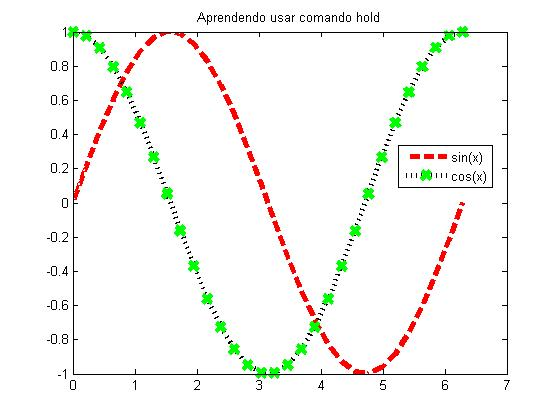
\includegraphics[scale=0.4]{grafico4.jpg}
\caption{Fun\c{c}\~oes novas em gr\'afico antigo.}
\label{fig:graf_bd4}
\end{figure}	

	Observe que podemos acrescentar um quarto argumento no plot, ou seja, al\'em de passar o par de vetores, a descri\c{c}\~ao das cores, tipos de linhas e marcadores, tamb\'em posso especificar a grossura da linha e dos marcadores, como o exemplo mostrou.

	Outra vantagem de trabalhar com Matlab \'e que esses detalhes podem ser editados na janela \textit{Figure}, como j\'a dito anteriormente. \'E poss\'{\i}vel passar somente em {\tt plot(x,y)} e acrescentar o resto dos detalhes na janela Figure.
	
\subsection{Figura M\'ultiplas}	
	
	Uma janela \textit{Figure} n\~ao precisa conter necessariamente um gr\'afico, isto \'e, podemos tratar \textit{Figure} como uma matriz de gr\'aficos que v\~ao guardando subgr\'aficos. Os subgr\'aficos s\~ao numerados da esquerda para a direita, primeiro na linha superior, depois na segunda linha e assim por diante. Por exemplo:

\begin{verbatim}	
>> x = linspace(0,2*pi,30);
>> y = sin(x);
>> z = cos(x);
>> a = 2*sin(x).*cos(x);
>> b = sin(x)./cos(x);
>> subplot(2,2,1)
>> plot(x,y), axis([0 2*pi -1 1]), title(`sin(x)')
>> subplot(2,2,2)
>> plot(x,z), axis([0 2*pi -1 1]), title(`cos(x)')
>> subplot(2,2,3)
>> plot(x,a), axis([0 2*pi -1 1]), title(`2sin(x)cos(x)')
>> subplot(2,2,4)
>> plot(x,b), axis([0 2*pi -1 1]), title(`sin(x)/cos(x)')
\end{verbatim}
\newpage
\begin{figure}[!h]
\centering
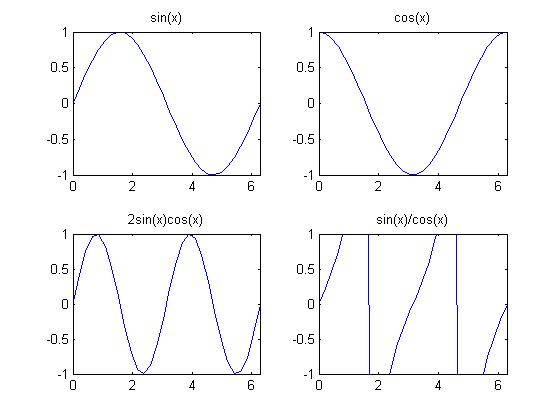
\includegraphics[scale=0.4]{grafico5.jpg}
\caption{Plotando subgr\'aficos.}
\label{fig:graf_bd5}
\end{figure}	

\subsection{Outra maneira de fazer gr\'aficos}
	Quando quiser plotar um gr\'afico e para n\~ao perder tempo calculando o vetor $y = f(x)$, ent\~ao, podemos recorrer ao comando {\tt fplot}, que recebe a fun\c{c}\~ao para calcular o vetor $y$ e um vetor que representa o eixo das abscissas. Mas lembre-se, ao usar {\tt fplot}, voc\^e est\'a passando uma fun\c{c}\~ao como argumento, ent\~ao nesse caso, \'e preciso trabalhar recomendavelmente com function\_handle.

\begin{verbatim}	
>> fplot(@(x) x^2-1,[-0.5 3],`g-.')
>> hold off
>> fplot(@exp,[-0.5 3],`r--')
>> hold on
>> fplot(@sin,[-0.5 3],`b:')
>> fplot(@(x) x^2-1,[-1.5 3],`g-.')
>> title(`Aprendendo a usar comando fplot')
\end{verbatim}

\begin{figure}[!h]
\centering
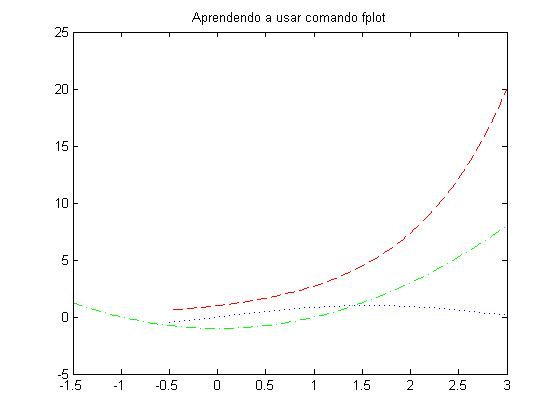
\includegraphics[scale=0.4]{grafico6.jpg}
\caption{Gr\'afico plotado por {\tt fplot}.}
\label{fig:graf_bd6}
\end{figure}	

\subsection{Mais coisas sobre plotar gr\'aficos}

	Existem outros gr\'aficos, com o de barras ou em forma de pizza, que n\~ao s\~ao provenientes de fun\c{c}\~oes nem de lista de pares ordenados. Mas mesmo assim, o Matlab consegue fazer esses tipos de gr\'afico.
	
\begin{table}[h]
\centering
\begin{tabular}{|l|l|} \hline	
\textbf{Fun\c{c}\~ao} & \textbf{Descri\c{c}\~ao} \\ \hline
{\tt plot} 						&	Gr\'afico Linear. \\ \hline
{\tt loglog} 					&	Gr\'afico Log-log. \\ \hline
{\tt semilogx} 				& Gr\'afico log-normal no eixo x. \\ \hline
{\tt semilogy} 				& Gr\'afico log-normal no eixo y. \\ \hline
{\tt polar} 					& Gr\'afico em coordenadas polares.  \\ \hline
{\tt grid on} 				& Ativa visibilidade das linhas de grade. \\ \hline
{\tt grid off} 				& Desativa visibilidade das linhas de grade. \\ \hline
{\tt area} 						& Hachura o gr\'afico.  \\ \hline
{\tt bar} 						& Gr\'afico de barras. \\ \hline
{\tt barh} 						& Gr\'afico de barras horizontais. \\ \hline
{\tt errorbar} 				& Gr\'afico linear com barras de erro.  \\ \hline
{\tt fplot} 					& Gr\'afico de uma fun\c{c}\~ao.  \\ \hline
{\tt hist} 						& Histograma.  \\ \hline
{\tt pie} 						& Gr'afico em forma de pizza.  \\ \hline
{\tt ribbom} 					& Gr\'afico linear com linhas bidimensionais em faixas.  \\ \hline
{\tt scatter} 				& Gr\'afico de dispers\~ao.  \\ \hline
{\tt stairs} 					& Gr\'afico de escada. \\ \hline
\end{tabular}
\caption{Fun\c{c}\~oes relacionadas com gr\'afico bidimensionais.}
\label{tab:lista_func_graf_bd}
\end{table}
	
\newpage
	
\section{Gr\'aficos Tridimensionais}

	Quando apresentamos vetores e, em seguida, matrizes, foi comentado que os comandos de vetor foram adaptados para matrizes. No caso de gr\'aficos, acontecer\'a a mesma situa\c{c}\~ao, isto \'e, os comandos de gr\'aficos tridimensionais ser\~ao como uma extens\~ao dos comandos de gr\'aficos bidimensionais.

\subsection{Gr\'aficos de Linhas}	
		A fun\c{c}\~ao {\tt plot} dos gr\'aficos bidimensionais \'e estendido para o {\tt plot3} para fazer gr\'aficos tridimensionais. Em {\tt plot3}, devemos apresentar uma tripla de vetores para podermos fazer o gr\'afico, no entanto, podemos acrescentar os argumentos extras para adicionar os detalhes de tipos de linhas, marcadores, cores, tamanho da letra etc. Vejamos os exemplos: 

\begin{verbatim}	
>> t = linspace(0,10*pi,100);
>> plot3(sin(t),cos(t),t)
>> grid on
>> xlabel(`sin(t)'),ylabel(`cos(t)'),zlabel(`t')
>> text(0,0,0,`Origem')
>> title(`Aprendendo Graficos Tridimensionais')
\end{verbatim}

\begin{figure}[!h]
\centering
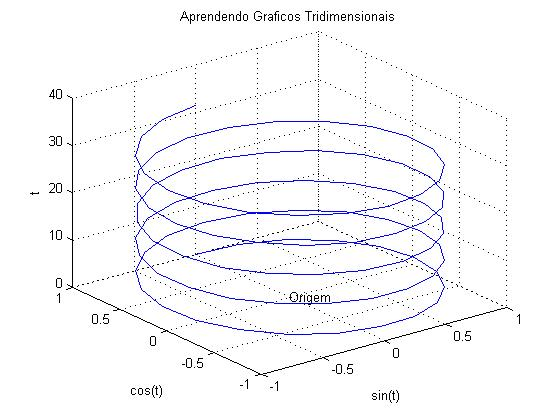
\includegraphics[scale=0.4]{grafico7.jpg}
\caption{O primeiro exemplo de gr\'afico tridimensional.}
\label{fig:graf_td7}
\end{figure}		

\begin{verbatim}	
>> x = linspace(-20,20); y = linspace(-20,20);
>> plot3(x,y,x.^2+y.^2,`r--',`LineWidth',3)
>> xlabel(`eixo-x'),ylabel(`eixo-y'),zlabel(`eixo-z')
>> title(`Outro exemplo para comando plot3')
>> grid on
\end{verbatim}

\newpage
\begin{figure}[!h]
\centering
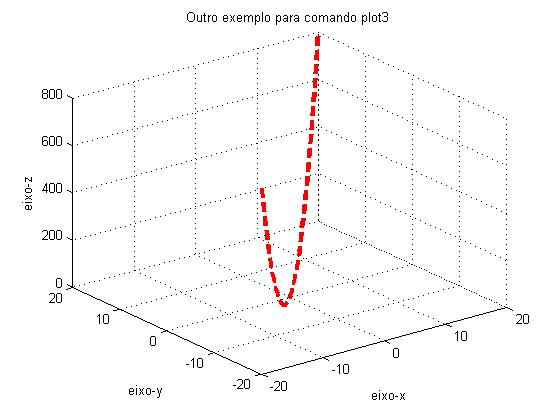
\includegraphics[scale=0.4]{grafico8.jpg}
\caption{Segunda exemplo de gr\'afico tridimensional.}
\label{fig:graf_td8}
\end{figure}	

\subsection{Fun\c{c}\~oes Escalares de Duas Vari\'aveis e o Gr\'afico de Rede}
	Pelo \'ultimo exemplo dado, encontramos a limita\c{c}\~ao do comando {\tt plot3}, que s\'o plota linhas. Para plotar uma fun\c{c}\~ao $z = f(x,y)$, o Matlab precisa receber uma matriz de todos os pontos do produto cartesiano do eixo-x com o eixo-y para poder calcular $z(x,y)$.
	
	Dados os vetores da coordenada do eixo x e y, o comando {\tt meshgrid(x,y)} realiza o produto cartesiano de eixo-x $\times$ eixo-y. Da\'{\i}, finalmente podemos plotar a superf\'{\i}cie usando o comando {\tt mesh(X,Y,Z)}. Por exemplo:

\begin{verbatim}	
>> x = linspace(-20,20); y = linspace(-20,20);
>> [X,Y] = meshgrid(x,y);
>> Z = (X+Y).^2;
>> mesh(X,Y,Z);
>> title(`Aprendendo a usar comando meshgrid e mesh')
\end{verbatim}

\begin{figure}[!h]
\centering
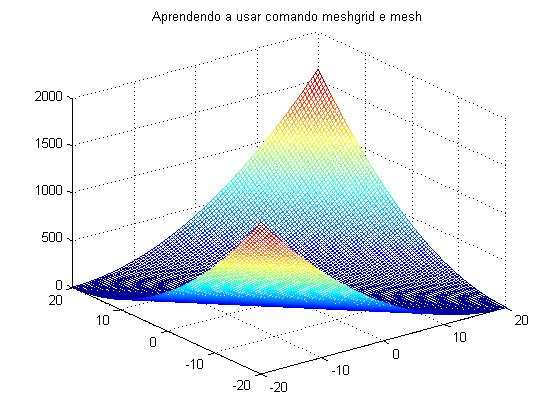
\includegraphics[scale=0.4]{grafico9.jpg}
\caption{Primeiro gr\'afico com {\tt meshgrid} e {\tt mesh}.}
\label{fig:graf_td9}
\end{figure}	

Mais um exemplo:

\begin{verbatim}	
>> Z2 = X.^2+Y.^2;
>> mesh(X,Y,Z2);
>> title(`Mais um exemplo com meshgrid e mesh')
\end{verbatim}

\begin{figure}[!h]
\centering
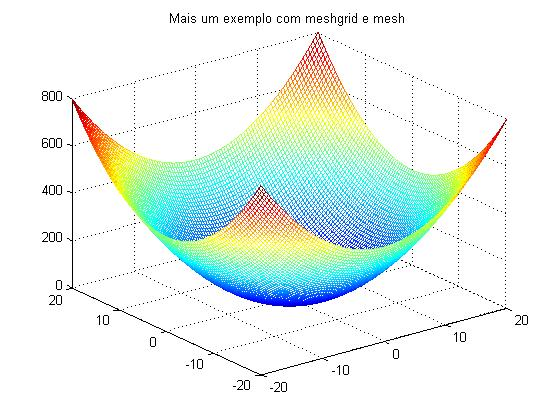
\includegraphics[scale=0.4]{grafico10.jpg}
\caption{Outro gr\'afico com {\tt meshgrid} e {\tt mesh}.}
\label{fig:graf_td10}
\end{figure}	

\subsection{Gr\'afico de Superf\'{\i}cie}

	Observe que o gr\'afico de rede obtido com o mesh \'e um gr\'afico todo furado. Nesta se\c{c}\~ao, vamos aprender como contruir uma superf\'{\i}cie todo preenchido com o comando surf.
	
\begin{verbatim}
>> x = linspace(-20,20); y = linspace(-20,20);
>> [X,Y] = meshgrid(x,y);
>> Z = (X+Y).^2;
>> mesh(X,Y,Z); title(`Grafico de rede criado pelo mesh')
>> surf(X,Y,Z); title(`Grafico de supreficie criado pelo surf')
\end{verbatim}	

\begin{figure}[!h]
\centering
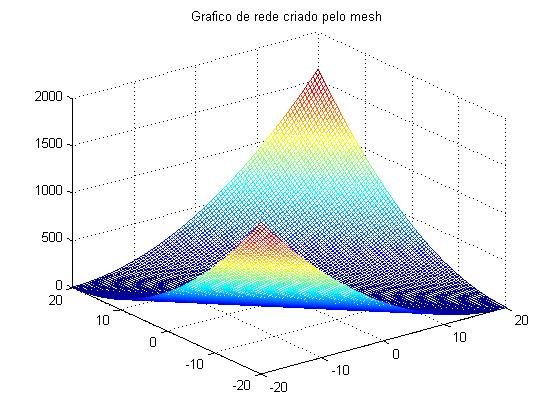
\includegraphics[scale=0.4]{grafico11.jpg}
\caption{Uma gr\'afico de rede.}
\label{fig:graf_td11}
\end{figure}	

\begin{figure}[!h]
\centering
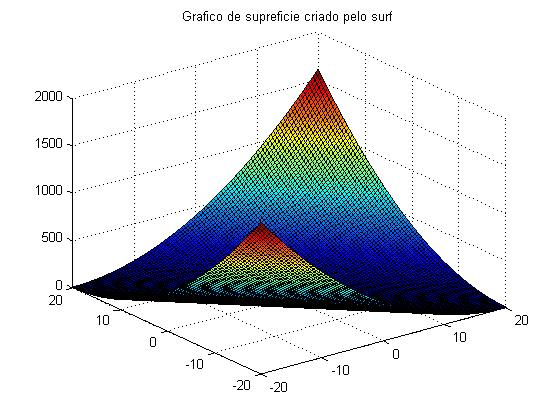
\includegraphics[scale=0.4]{grafico12.jpg}
\caption{Um gr\'afico de superf\'{\i}cie.}
\label{fig:graf_td12}
\end{figure}	

\subsection{Curvas de N\'{\i}vel}
	Nos gr\'aficos tridimensionais, podemos plotar tamb\'em as curvas de n\'{\i}vel. Como se n\~ao bastasse, o Matlab ainda nos d\'a a op\c{c}\~ao de plotar as curvas de n\'{\i}vel bi e tridimensionais. Veja os exemplos:

\begin{verbatim}
>> x = linspace(-20,20); y = linspace(-20,20);
>> [X,Y] = meshgrid(x,y);
>> Z = (X+Y).^2;
>> contour(X,Y,Z,20);
>> title(`Grafico de Curva de Nivel Bidimendional')
\end{verbatim}	

\begin{figure}[!h]
\centering
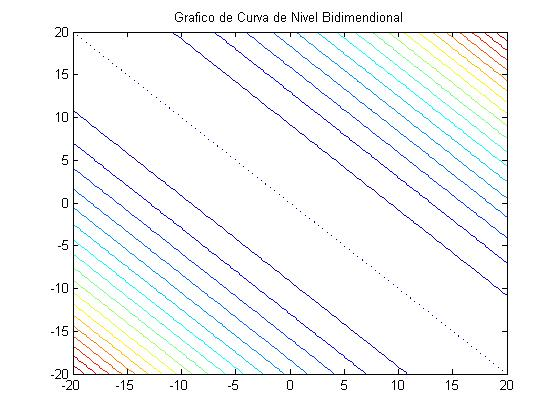
\includegraphics[scale=0.4]{grafico13.jpg}
\caption{Curva de n\'{\i}vel bidimensional.}
\label{fig:graf_td13}
\end{figure}	

\begin{verbatim}
>> Z2 = X.^2+Y.^2;
>> contour3(X,Y,Z2,20);
>> title(`Grafico de Curva de Nivel Tridimensional')
\end{verbatim}	

\newpage
\begin{figure}[!h]
\centering
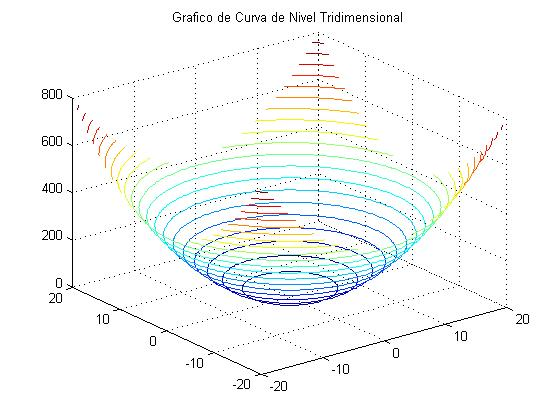
\includegraphics[scale=0.4]{grafico14.jpg}
\caption{Curva de n\'{\i}vel tridimensional.}
\label{fig:graf_td14}
\end{figure}	

	Tamb\'em podemos plotar gr\'aficos bi e tridimensionais com legenda, atrav\'es do comando {\tt clabel}.

\begin{verbatim}
>> [X3,Y3,Z3] = peaks;
>> C = contour(X3,Y3,Z3,10);
>> clabel(C);
>> title(`Grafico de curvas de nivel com legendas')
\end{verbatim}	

\begin{figure}[!h]
\centering
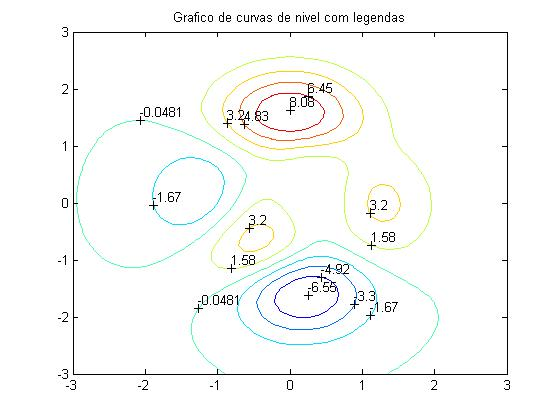
\includegraphics[scale=0.4]{grafico15.jpg}
\caption{Um dos gr\'aficos de curvas de n\'{\i}vel produzido por {\tt clabel}.}
\label{fig:graf_td15}
\end{figure}	

\begin{verbatim}
>> [C,h] = contour(X3,Y3,Z3,8);
>> clabel([C,h]);
>> clabel(C,h);
>> title(`Grafico de curvas de nivel com legendas inserida nas curvas')
\end{verbatim}	

\newpage
\begin{figure}[!h]
\centering
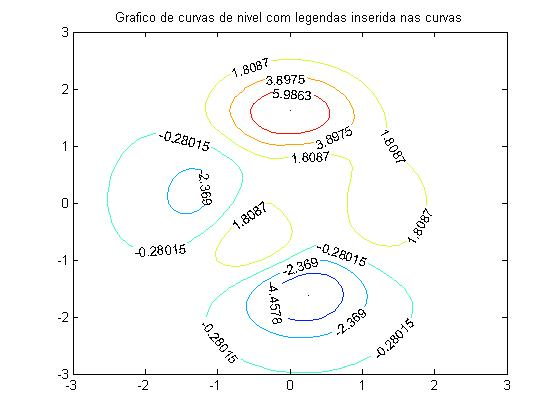
\includegraphics[scale=0.4]{grafico16.jpg}
\caption{Segunto tipo de gr\'aficos de curvas de n\'{\i}vel produzido por {\tt clabel}.}
\label{fig:graf_td16}
\end{figure}	

\subsection{Mais Comandos sobre Gr\'aficos Tridimensionais}
\begin{table}[h]
\centering
\begin{tabular}{|l|l|} \hline	
\textbf{Fun\c{c}\~ao} & \textbf{Descri\c{c}\~ao} \\ \hline
{\tt plot3} 					&	Tra\c{c}a linha e pontos no espa\c{c}o tridimensional. \\ \hline
{\tt mesh}  					& Superf\'{\i}cie na forma de uma rede. \\ \hline
{\tt meshc} 					& Gr\'afico de rede com curvas de n\'{\i}vel por baixo. \\ \hline
{\tt surf} 						& Gr\'afico de superf\'{\i}cie. \\ \hline
{\tt surfc} 					& Gr\'afico de superf\'{\i}cie com curvas de n\'{\i}vel por baixo. \\ \hline
{\tt hidden on}				& Remove as linhas invis'iveis da malha. \\ \hline
{\tt hidden off}			& N\~ao remove as linhas invis'iveis da malha. \\ \hline
{\tt grid on} 				& Inclui linhas de grade.  \\ \hline
{\tt grid off} 				& N\~ao inclui linhas de grade.  \\ \hline
{\tt axis} 						& Controla a apar\^encia e a escala usada nos eixos.  \\ \hline
{\tt hold} 						& Mant\'em na tela o gr\'afico atual.  \\ \hline
{\tt subplot} 				& Cria v\'arios eixos em uma janela \textit{Figure}.  \\ \hline
{\tt title} 					& T\'{\i}tulo do gr\'fico.  \\ \hline
{\tt xlabel} 					& Legenda do eixo-x.  \\ \hline
{\tt ylabel} 					& Legenda do eixo-y.  \\ \hline
{\tt zlabel} 					& Legenda do eixo-z.  \\ \hline
{\tt text} 						& Coloca texto no gr\'afico.  \\ \hline
{\tt contour} 				& Gr\'afico de curvas de n\'{\i}vel.  \\ \hline
{\tt contour3} 				& Gr\'afico de faixas de n\'{\i}vel.  \\ \hline
{\tt clabel} 					& Legendas de curvas de n\'{\i}vel.  \\ \hline
\end{tabular}
\caption{Fun\c{c}\~oes relacionadas a gr\'aficos tridimensionais.}
\label{tab:lista_func_trid}
\end{table}






%\begin{verbatim}\end{verbatim}
%\line(1,0){200}
	
	



\end{document}
